%----------------------------------------------------------------
%
%  File    :  thesis.tex
%
%  Authors :  David Walser, Wien, Austria
% 
%  Created :  08 Feb 2022
% 
%  Changed :  08 Feb 2022
%
%  For suggestions and remarks write to: sebastian.ukleja@fh-campuswien.ac.at 
%----------------------------------------------------------------

% --- Setup for the document ------------------------------------

%Class for a book like style:
\documentclass[11pt,a4paper,oneside]{scrbook}
%For a more paper like style use this class instead:
%\documentclass[11pt,a4paper,oneside]{thesis}

%input encoding for windows in utf-8 needed for Ä,Ö,Ü etc..:
\usepackage[utf8]{inputenc}
%input encoding for linux: 
%\usepackage[latin1]{inputenc}
%input encoding for mac:
%\usepackage[applemac]{inputenc}

\usepackage[ngerman]{babel}
%for english use this instead:
%\usepackage[english]{babel}

%needed for font encoding
\usepackage[T1]{fontenc}

% want Arial? uncomment next two lines...
%\usepackage{uarial}
%\renewcommand{\familydefault}{\sfdefault}

%some formatting packages
\usepackage[bf,sf]{subfigure}
\renewcommand{\subfigtopskip}{0mm}
\renewcommand{\subfigcapmargin}{0mm}

%For better font resolution in pdf files
\usepackage{lmodern}

\usepackage{url}


%\usepackage{latexsym}

\usepackage{geometry} % define pagesize in more detail

% --- Settings for header and footer ---------------------------------
\usepackage{scrlayer-scrpage}
\clearscrheadfoot
\pagestyle{scrheadings}
\automark{chapter}

%Left header shows chapter and chapter name, will not display on first chapter page use \ihead*{\leftmark} to show on every page
\ihead{\leftmark} 	
%\ohead*{\rightmark}	%optional right header
\ifoot*{David Walser}		%left footer shows student name
\ofoot*{\thepage}		%right footer shows pagination
%---------------------------------------------------------------------

\usepackage{colortbl} % define colored backgrounds for tables

\usepackage{courier} %for listings
\usepackage{listings} % nicer code formatting
\lstset{basicstyle=\ttfamily,breaklines=true}

\usepackage{graphicx}
  \pdfcompresslevel=9
  \pdfpageheight=297mm
  \pdfpagewidth=210mm
  \usepackage[         % hyperref should be last package loaded
    pdftex, 		   % needed for pdf compiling, DO NOT compile with LaTeX
    bookmarks,
    bookmarksnumbered,
    linktocpage,
    pagebackref,
    pdfview={Fit},
    pdfstartview={Fit},
    pdfpagemode=UseOutlines,                 % open bookmarks in Acrobat
  ]{hyperref}
\DeclareGraphicsExtensions{.pdf,.jpg,.png}
\usepackage{bookmark}

\usepackage[title]{appendix}

\usepackage{wrapfig}
%paper format
\geometry{a4paper,left=30mm,right=25mm, top=30mm, bottom=30mm}

\setlength{\parskip}{3pt plus 1pt minus 0pt}       % vert. space before a paragraph

\setcounter{tocdepth}{1}        % lowest section level entered in ToC
\setcounter{secnumdepth}{2}     % lowest section level still numbered

%Start of your document beginning with title page
\begin{document}
\frontmatter

% --- Main Title Page ------------------------------------------------
\begin{titlepage}
\begin{picture}(50,50)
\put(-70,40){\hbox{
\includegraphics{images/logo.png}}}
\end{picture}

\vspace*{-5.8cm}

\begin{center}

\vspace{6.2cm}

\hspace*{-1.0cm} {\LARGE \textbf{Bildähnlichkeitserkennung von Markenlogos mithilfe von Machine Learning \\}}
\vspace{0.2cm}
\hspace*{-1.0cm} Untertitel \\

\vspace{2.0cm}

\hspace*{-1.0cm} { \textbf{Masterarbeit\\}}

\vspace{0.65cm}

\hspace*{-1.0cm} Eingereicht in teilweiser Erfüllung der Anforderungen zur Erlangung des akademischen Grades: \\

\vspace{0.65cm}

\hspace*{-1.0cm} \textbf{Master of Science in Engineering\\}

\vspace{0.65cm}

\hspace*{-1.0cm} an der FH Campus Wien \\
\vspace{0.2cm}
\hspace*{-1.0cm} Studienfach: Software Design and Engineering \\

\vspace{1.6cm}

\hspace*{-1.0cm} \textbf{Autor:} \\
\vspace{0.2cm}
\hspace*{-1.0cm} David Walser \\

\vspace{0.7cm}

\hspace*{-1.0cm} \textbf{Matrikelnummer:}\\
\vspace{0.2cm}
\hspace*{-1.0cm} 01609388 \\

\vspace{0.7cm}

\hspace*{-1.0cm} \textbf{Betreuer:} \\
\vspace{0.2cm}
\hspace*{-1.0cm} FH-Prof. DI Dr. Igor Miladinovic \\

\vspace{0.7cm}

% Reviewer if needed:
%\hspace*{-1.0cm} \textbf{Reviewer: (optional)} \\
%\vspace{0.2cm}
%\hspace*{-1.0cm} Titel Vorname Nachname \\


\vspace{1.0cm}

\hspace*{-1.0cm} \textbf{Datum:} \\
\vspace{0.2cm}
\hspace*{-1.0cm} 02.02.2022 \\

\end{center}
\end{titlepage}

\newpage
\setcounter{page}{1}

\vspace*{16cm}

% --- Declaration of authorship ----------------------------------------------------
\hspace*{-0.7cm} \underline{Erklärung der Urheberschaft:}\\\\
Ich erkläre hiermit diese Masterarbeit eigenständig verfasst zu haben. Ich habe keine anderen Quellen, als die in der Arbeit gelisteten verwendet, noch habe ich jegliche unerlaubte Hilfe in Anspruch genommen\\\\
Ich versichere diese Masterarbeit in keinerlei Form jemandem Anderen oder einer anderen Institution zur Verfügung gestellt zu haben, weder in Österreich noch im Ausland.\\\\
Weiters versichere ich, dass jegliche Kopie (gedruckt oder digital) identisch ist.
\\\\\\
Datum: \hspace{6cm} Unterschrift:\\

% --- English Abstract ----------------------------------------------------
\cleardoublepage
\chapter*{Abstract}
(E.g. ``This thesis investigates...'')


% --- German Abstract ----------------------------------------------------

\cleardoublepage
\chapter*{Kurzfassung}
(Z.B. ``Diese Arbeit untersucht...'')

% --- Abbrevations ----------------------------------------------------
\newpage\noindent
\chapter*{Abkürzungen}
\vspace{0.65cm}

\begin{table*}[htbp]
		\begin{tabular}{ll}
			ÖPA & Österreichisches Patentamt \\
			KNN & künstliches neuronales Netzwerk \\
			CNN & convolutional neural network \\
			ARP & Address Resolution Protocol \\
			GPRS & General Packet Radio Service \\
			GSM  &  Global System for Mobile communication \\
			WLAN & Wireless Local Area Network \\
		\end{tabular}
\end{table*}

% --- Key terms ----------------------------------------------------
\newpage
\chapter*{Schlüsselbegriffe}
\vspace{0.65cm}

\begin{itemize}
	\setlength{\itemsep}{0pt}
	\item[] GSM
	\item[] Mobilfunk
	\item[] Zugriffsverfahren
\end{itemize}

% --- Table of contents autogenerated ------------------------------------
\newpage
\tableofcontents
\thispagestyle{empty}

% --- Begin of Thesis ----------------------------------------------------
\mainmatter
\chapter{Einführung}
\label{chap:intro}
\section{Problembeschreibung}
\label{sec:Problembeschreibung}
Für uns Menschen ist es eine ziemlich einfache Aufgabe zu ermitteln ob ein Bild ähnlich zu einem anderen ist oder nicht. 
Wir erkennen alle Möglichen Merkmale eines Bildes, wie Farben, Texte oder Muster, ohne große Schwierigkeiten.
Es stellt jedoch eine Herausforderung dar, wenn ein Bild mit 400.000 anderen Bildern verglichen und auf ähnlichkeit geprüft werden soll.

Im Jahre 2020 wurden 6260 neue Marken beim österreichischen Patentamt angemeldet \cite{oepastatistik2020}.
Die meisten dieser Marken werden in Kombination mit einem Bild, auch Logo genannt, registriert.
Damit es bei einer Neuanmeldung nicht zu einer unmittelbaren Verwechslungsgefahr mit bereits bestehenden Marken kommt, bietet das österreichische Patentamt einen Dienst an, bei dem Daten zu einer Marke angegeben werden, und überprüft wird, ob es Ähnlichkeiten mit bereits angemeldeten Marken gibt \cite{oepamarkenaehnlichkeitsrecherche}. 
Ein Hauptbestandteil dieser Ähnlichkeitsrecherche ist die Überprüfung von Ähnlichkeiten der Logos. 

\section{Motivation und Ziel}
\label{sec:motivationundziel}
Machine Learning ist ein aufkommendes und zukunftsweisendes Thema.
Laut einer Studie aus 2017 wurde ein Wachstum des machine learning Marktes von 1.03 Milliarden \$ in 2016 auf 8.81 Milliarden \$ im Jahre 2022 erwartet, was einer Wachstumsrate von 44.1\% entsrpicht \cite{researchandmarkets}.
Eines der Hauptprobleme im Bereich Computer Vision ist es ähnliche Bilder in großen und unstrukturierten Kollektionen zu finden.
Es kann ein sehr zeitaufwändiges Verfahren sein, da hier viele Bilder getestet werden müssen um eine Übereinstimmung zwischen Parren zu finden \cite{siameseieee}. 
Technologisch gesehen ist der mit dieser Masterarbeit verbundene Prototyp eine große Herausforderung, da zur Umsetzung allerneuste Technologien und Frameworks benötigt werden.
Eine weitere Herausforderung wird es sein, wie genau die vom österreichischen Patentamt dankenswerter weise zur Verfügung gestellten Daten zu analysieren und kategorisieren sind.
Ziel dieser Masterarbeit ist es das Patentamt bei der Ähnlichkeitsrecherche zu unterstützen, in dem ein Prototyp entwickelt wird, welcher Ähnlichkeiten bei Bildern erkennt.
Außerdem soll diese Masterarbeit einen Überblick über Machine Learning, mit Fokus auf Bildverarbeitung, enthalten.
Daraus ergibt sich die folgende Forschungsfrage \begin{quotation}Welche Unterschiede weisen verschiedene ML Algorithmen auf, im Bezug auf Erkennungsrate einer Ähnlichkeitsüberprüfung von Bildern?\end{quotation} zu beantworten.

tbd. more!

\chapter{Machine learning}
\label{chap:machinelearning}
Für viele Firmen ist machine Learning bereits der meist benutzte Bereich aus dem Feld der künstlichen Intelligenz \cite{imageprocessingnanonets}.
Machine Learning ist die Wissenschaft und Kunst Computern das Lernen anhand von Daten zu ermöglichen \cite{geron2019hands-on} und ist ein Anwendungsgebiet von künstlicher Intelligenz welches bereits seit vielen Jahren die Forschung und Wirtschaft unterstützt \cite{datasolutml}. 
"Machinelles Lernen ist ein Oberbegriff für die "künstliche" Generierung von Wissen aus Erfahrung: Ein künstliches System lernt aus Beispielen und kann diese nach Beendigung der Lernphase verallgemeinern." \cite{wikipediaml}
Muster und Gesetzmäßigkeiten werden aus den Trainignsdaten erkannt, woraus ein staistisches Modell erzeug wird \cite{wikipediaml}.
Dieser Prozess wird als Modelltraining bezeichnet und ist ein iterativer Prozess, welcher oft mehrfach durchlaufen wird, bis die Qualität des Ergebnis zufriedenstellend ist \cite{datasolutml}.
Aus dem Erlernen und Analysieren der historischen Daten kann ein Ergebnis für neue und unbekannte Daten prognostiziert werden, ohne explizit darauf programmiert zu sein \cite{techtargetml}. 
\begin{figure}[htbp]
	\centering
		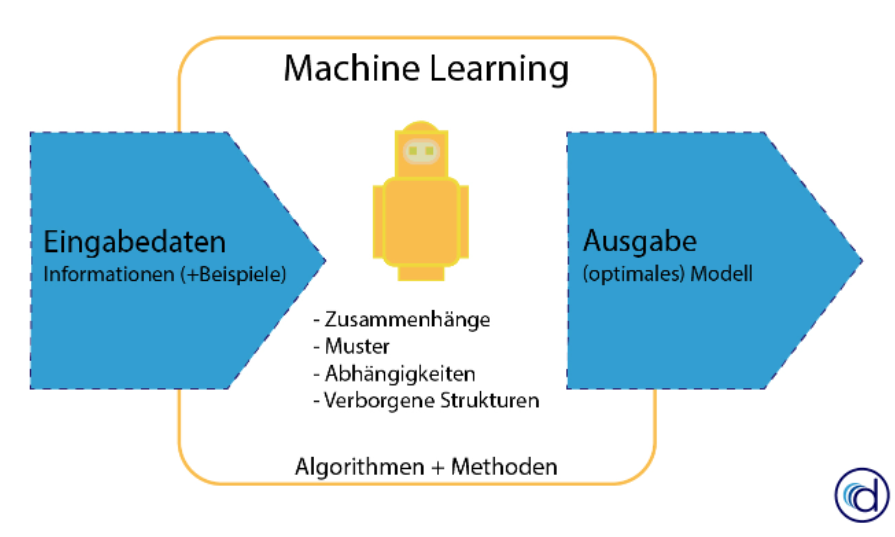
\includegraphics[height=5cm]{images/machine_learning.png}
	\caption{Machine Learning nimmt Eingabedaten mit Beispielen und lernt daraus, um für die Zukunft Prognosen zu machen \cite{datasolutml}}
	\label{fig:machine_learning}
\end{figure}

Ein Alltag ohne dem Interagieren mit Machine Learning ist heutzutage kaum mehr wegzudenken.
Bei der Benutzung von sozialen Medien, online Shopping oder Bankdiensten kommt Machine Learning zum Einsatz \cite{oracleml} und bereits seit den 1990er Jahren beeinflusst Machine Learning in Form des Spam Filters das Leben vieler \cite{geron2019hands-on}. 
Netflix bietet mithilfe von Machine Learning personalisierte Film und Serienempfehlungen an, und zusätzlich unterstützt Machine Learning bei der Optimierung der Produktion von Filmen und TV Shows \cite{netflixml}.  
Facebooks Algorithmus kann bereits mit 100 bis 150 Likes die Persöhnlichlkeit einer Person genauer beschreiben als deren Familienmitglieder oder Freunde \cite{facebookml}. 
Die Grundlage für Machine Learning bilden Algorithmen, welche sich in folgende Arten aufteilen lassen \cite{oracleml}: 
\begin{itemize}
	\item supervised learning,
	\item unsupervised learning,
	\item semi-supervised learning und
	\item reinforcement learning.
\end{itemize}

\section{Supervised Machine Learning}
\label{sec:supervised}
Supervised Machine Learning, im Deutschen übersetzt überwachtes Lernen, ist die am häufigsten angewendete Algorithmusart \cite{oracleml}.
Ähnlich wie in der Schule wenn unter Aufsicht des Lehrers oder der Lehrerin geprüft wird, ob ein Problem richtig oder falsch gelöst wird, ist die Situation bei supervised Machine Learning Algorithmen.
Dem Algorithmus wird ein gelabelter Datensatz zum Lernen zur Verfügung gestellt, somit weiß der Algorithmus für jeden Datensatz die richtige Lösung \cite{intellipaatml}. 
Ein gelabelter Datensatz kann z.B. ein Bild von einem Tier sein, wobei hier zusätzlich auch die Information über ein Feature mitgegeben wird, wie z.B. die Art des Tieres oder das Gewicht des Tieres (siehe Abbildung ~\ref{fig:labeled_vs_unlabeled}).
Das Label ist die Information über ein Feature welche der Algorithmus später vorhersagen will \cite{grokkingml}.
\begin{figure}[htbp]
	\centering
		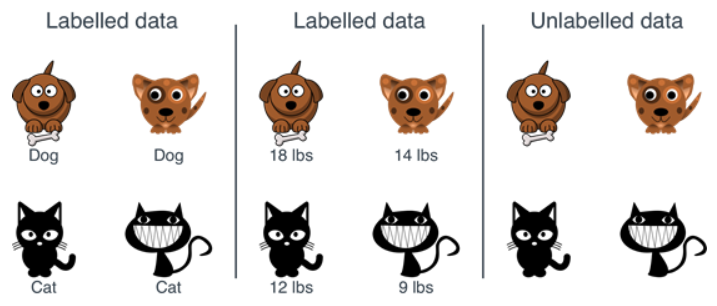
\includegraphics[height=4cm]{images/labeled_vs_unlabeled.png}
	\caption{Labeled vs unlabeled Data \cite{grokkingml}}
	\label{fig:labeled_vs_unlabeled}
\end{figure}
Folgende Algorithmen sind Beispiele für supervised Learning \cite{geron2019hands-on}:
\begin{itemize}
	\item k-Nearest Neighbors
	\item Naive Bayes
	\item Linear Regression
	\item Logistic Regression
	\item Support Vector Machines (SVMs)
	\item Decision Trees und Random Forests
	\item Neuronale Netzwerke (wobei diese auch unsupervised oder semisupervised sein können) 
\end{itemize}
Klassifizierung und Regression sind klassische Anwendungsgebiete für supervised Learning \cite{geron2019hands-on}.
\subsection{Klassifizierung}
Bei Klassifizierungsproblemen geht es darum einen Status vorherzusagen \cite{grokkingml}, wie z.B. zu welcher Klasse oder Gruppe die Inputdaten gehören \cite{intellipaatml}. 
Der Spam Filter ist ein gutes Beispiel für Klassifizierung, hierbei handelt es sich um zwei Klassen: Spam und nicht Spam.
Der Algorithmus bekommt E-Mails zum Lernen, welche als Spam E-Mail oder normale E-Mail gelabelt sind, um somit für neue E-Mails herauszufinden, ob diese Spam E-Mails sind \cite{geron2019hands-on}. 
\subsection{Regression}
Regression ist ein Fachgebiet der Statistik und ist eine Methode um die Beziehung zwischen unabhängigen Variablen oder Merkmalen und einer abhänigen Variable oder einem Ergebnis zu verstehen.
Sobald die Beziehung zwischen unabhängigen und abhängigen Variablen geschätzt wurde, können die Ergebnisse vorhergesagt werden \cite{unsupervisedibm}. 
Bei Regressionsproblemen geht es um kontinuierliche Daten \cite{intellipaatml} und darum eine Zahl vorherzusagen, wie z.B. das Vorhersagen von Aktienkursen \cite{grokkingml} oder von Grundstückspreisen \cite{intellipaatml}.

\section{Unsupervised Machine Learning}
\label{sec:unsupervised}
Bei unsupervised Machine Learning, im Deutschen übersetzt unüberwachtes Lernen, handelt es sich um den Ansatz mit Datensätzen zu lernen, welche kein Label besitzen \cite{geron2019hands-on}.
Dies wird auch als selbst organisiertes Lernen bezeichnet \cite{intellipaatml}, da der Algorithmus ohne einen Lehrer oder eine Lehrerin lernt \cite{geron2019hands-on}. 
Da es sich hierbei um ungelabelte Datensätze handelt, besitzen diese nicht die Zielinformation, welche vorhergesagt werden soll \cite{grokkingml} und somit werden Zusammenhänge in den Daten \cite{unsuperviseddatasolut}, versteckte Muster oder Datengruppierungen von unsupervised Algorithmen erkennt, ohne dass menschliches Eingreifen erforderlich ist \cite{unsupervisedibm}.
\begin{figure}[htbp]
	\centering
		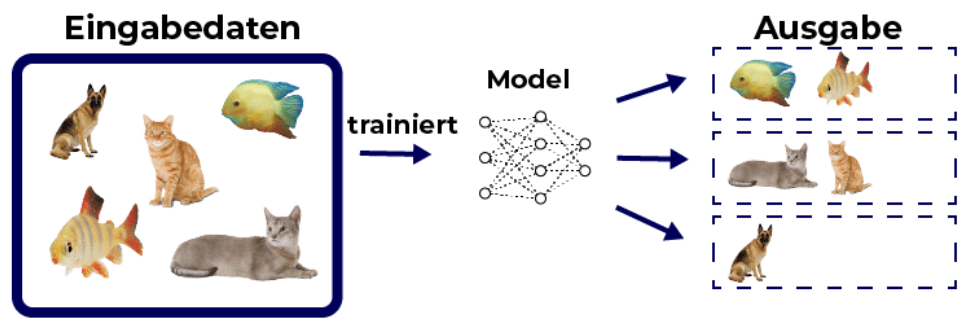
\includegraphics[height=4cm]{images/unsupervised.png}
	\caption{"Model trainiert ohne Zielvariable und findet eigenständig Muster und Zusammenhänge in den Daten" \cite{unsuperviseddatasolut}}
	\label{fig:unsupervised}
\end{figure}
Die Fähigkeit, Ähnlichkeiten und Unterschiede in Informationen zu entdecken, macht sie zur idealen Lösung für die explorative Datenanalyse, Kundensegmentierung und Bilderkennung.
Folgende Algorithmen sind Beispiele für unsupervised Learning \cite{geron2019hands-on}:
\begin{itemize}
	\item K-Means
	\item DBSCAN
	\item Hierarchical Cluster Analysis (HCA)
	\item Principal Component Analysis (PCA)
	\item Kernel PCA
	\item Locally-Linear Embedding (LLE)
	\item Apriori
	\item Eclat
\end{itemize}
Clustering, Assoziationsanalyse und Dimensionalitätsreduktion sind die drei Hauptaufgaben von unsupervised Machine Learning \cite{unsupervisedibm}.
\subsection{Clustering}
Beim Clustering geht es darum, die Population oder die Datenpunkte in eine Reihe von Gruppen aufzuteilen, so dass die Datenpunkte in denselben Gruppen anderen Datenpunkten in derselben Gruppe ähnlicher und den Datenpunkten in anderen Gruppen unähnlicher sind \cite{clusteringgeeks}.
Es werden ungelabelte Daten auf der Grundlage ihrer Ähnlichkeiten oder Differenzen in verschiedene Gruppen aufgeteilt \cite{unsupervisedibm}. 
Anwendungsgebiete für Clustering sind beispielsweise Bücher die je nach Titel und Inhalt in verschiedene Gruppen eingeteilt werden oder Pflanzen und Tiere welche in Spezies aufgeteilt werden (siehe Abbildung ~\ref{fig:unsupervised}) \cite{clusteringgeeks}.
\subsection{Assoziationsanalyse}
Die Assoziationsanalyse ist eine Methode um herauszufinden welche Muster (Beziehungen, Korrelationen, Strukturen, ...) es in den Datensätzen gibt \cite{associationmedium}.
Diese Methode wird häufig für Warenkorbanalysen verwendet, um ein besseres Verständis über die Beziehung zwischen den Produkten zu bekommen. 
Beispiele davon sind z.B. auf Amazon die \"{}Kunden, die diesen Artikel gekauft haben, kauften auch:\"{} Anzeige oder die Spotify "Discover Weekly" Playlist. \cite{unsupervisedibm}
\subsection{Dimensionalitätsreduktion}
Während mehr Daten grundsätzlich zu genaueren Ergebnissen führen können, so kann dies auch die Leistung von Algorithmen für machine Learning beeinträchtigen (z.B. overfitting) und die Visualisierung von Datensätzen erschweren \cite{unsupervisedibm}.
Bei der Dimensionalitätsreduktion geht es darum, die Variablen in den Daten auf die wesentlichen und zielführenden zu beschränken (z.B. werden redundante oder noise Features entfernt) \cite{unsuperviseddatasolut}, wobei die Integrität der Daten so weit wir möglich erhalten bleiben soll \cite{unsupervisedibm}.
Es kann für das bereinigen von Daten oder auch für das Hervorheben von Features verwendet werden, da die Daten dabei von hochdimensionalem Featureraum in niedrigdimensionalem Featureraum transformiert werden \cite{dimensionalityneptune}.
Ein Beispiel für Dimensionalitätsreduktion könnte die Redkution von zweidimensionale Eingabedaten in eindimansionale umzuwandeln.
%https://towardsdatascience.com/11-dimensionality-reduction-techniques-you-should-know-in-2021-dcb9500d388b

\section{Semi-supervised Learning}
\label{sec:semisupervised}
Um die Schwierigkeiten vom Erstellen von großen gelabelten Datensätzen entgegenzuwirken gibt es eine Methode bei der ein kleiner Anteil gelabelte Daten, der Großteil jedoch ungelabelte Daten sind.
Dieese Methode wird als semi-supervised Learning bezeichnet, welche die Benefits von unsupervised und supervised kombiniert \cite{semisuperviseddatarobot}. 
Der Algorithmus wird initial mit den wenig gelabelten Daten trainiert und kann somit iterativ mehr und mehr an die ungelabelten Daten angewandt werden.
Self-training und Co-training sind zwei Ansätze für semi-supervised learning. \cite{semisupervisedalexsoft}
\subsection{Self-training}
Self-training ist eines der einfachsten Beispiele für semi-supervised learning und ist ein Prozedere einen supervised learning Ansatz in semi-supervised umzuwandeln \cite{semisupervisedalexsoft}.
Der straightforward Ansatz wird anhand folgendem Beispiel erklärt:
\begin{enumerate}
	\item Die gelabelten Daten werden für das Trainieren des Models herangenommen \cite{selftrainingtowardsdatasience}.
	\item Dieses Model wird dann für die Vorhersage von ungelabelten Daten verwendet \cite{selftrainingtowardsdatasience}.
	\item Es werden Ergebnisse, welche dem zuvor bestimmten Kriterium entsprechen (z.B. >90\% accuracy), mit pseudo-labels verzehrt und mit den bereits gelabelten Daten kombiniert \cite{selftrainingtowardsdatasience}.
	\item Das Model wird nun mit dem neuen Pool an gelabelten Daten trainiert \cite{selftrainingtowardsdatasience}.
	\item Der ganze Prozess wird nun durchiteriert bis entweder alle Daten gelabelt sind oder die spezifizierte Maximalanzahl an Iterationen erreicht wird \cite{selftrainingtowardsdatasience}.
\end{enumerate}
Die Performance von dem Self-training Ansatz variiert von Datensatz zu Datensatz und es gilt abzuwägen ob sie im Vergeleich zu dem supervised Ansatz eine Verbesserung erzielt \cite{semisupervisedalexsoft}. 
Ein Anwendugsfall für Self-training könnte z.B. das Erkennen von Bildrotationen sein.
Es werden dabei z.B. Bilder in 90 Grad schritten rotiert, und durch Self-training wird herausgefunden um wieviel Grad es sich handelt.
% https://dasha.ai/en-us/blog/self-supervised-machine-learning

\subsection{Co-training}
Co-training ist eine verbesserte Version von Self-Training, die zum Einsatz kommt, wenn nur wenig gelabelte Daten verfügbar sind \cite{semisupervisedalexsoft}.
Bei dieser Methode benötigt es zwei Sichten auf die Daten \cite{cotrainingwiki} und basierend darauf werden zwei individuelle Klassifizierer trainiert \cite{semisupervisedalexsoft}.
Die zwei Ansichten sind verschiedene Gruppen von Features, welche jeweils Informationen für jede Instanz beinhalten \cite{semisupervisedalexsoft}.
Dies bewirkt dass beide Ansichten unabhängig sind und sie alleinstehend die Klasse einer Instanz vorhersagen können \cite{cotrainingwiki}.
Ein Anwendugsgebiet für Co-Training könnte die Klassifizierung von Webinhalten sein.
Der Inhalt einer Webseite kann in zwei Ansichten aufgeteilt werden: eine mit Wörtern, und die andere mit Verweistexten der Links, welche zu dieser Seite führen \cite{semisupervisedalexsoft}. 
Der Ablauf eines Co-Trainings sieht wie folgt aus:
\begin{enumerate}
	\item Für jede Ansicht werden die seperaten Models mit den gelabelten Daten trainiert \cite{semisupervisedalexsoft}.
	\item Die ungelabelten Daten werden hinzugefügt und mit pseudo-labels versehen \cite{semisupervisedalexsoft}.
	\item Die beiden Klasifizierer trainieren sich gegenseitig mit den pseudo-labels und es wird das höchste Konfidenzniveau angestrebt. Wenn z.B. der erste Klassifizierer das Label für einen Datensatz vorhersagt, während der andere einen Fehler macht, so werden die vom ersten Klassifizierer zugewiesenen pseudo-labels jene vom zweiten überschreiben und vice-versa. \cite{semisupervisedalexsoft}
	\item Zuletzt werden die beiden geupdaten Klassifizierer in zu einem kombiniert \cite{semisupervisedalexsoft}.
\end{enumerate}

\section{Reinforcement Learning}
\label{sec:reinforcement}
Reinforcement Learning, im Deutschen übersetzt Bestärkendes oder Verstärkendes Lernen, ist eine immer beliebter werdende Methode und  befasst sich damit intelligente Lösungen für komplexe Steuerungsprobleme zu finden \cite{reinforcementat}.
Das lernende System, welches in diesem Kontext \textit{Agent} genannt wird, beobachtet das Umfeld und führt dann Aktionen aus, für die es entweder Belohnungen oder Bestrafungen bekommt \cite{geron2019hands-on}.
\begin{figure}[htbp]
%\begin{wrapfigure}{r}{0.5\textwidth}
	\centering
		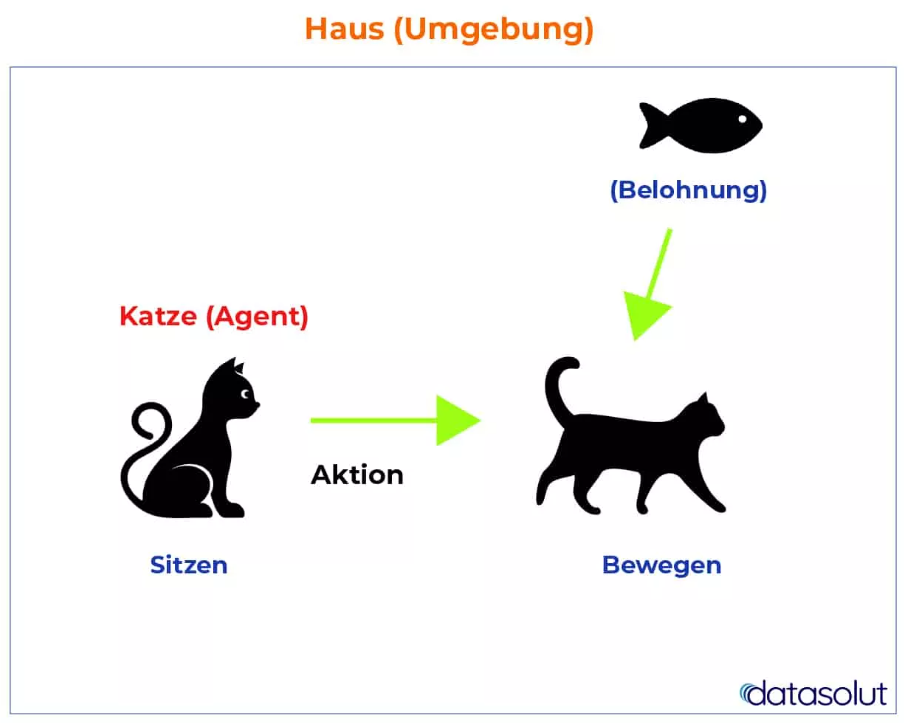
\includegraphics[height=6cm]{images/reinforcement.png}
	\caption{Beispiel von Reinforcement Learning \cite{reinforcementdatasolut}}
	\label{fig:reinforcement}
%\end{wrapfigure}
\end{figure}
Hierbei erlernt der Agent eigenständig welche Aktion für welche Situation am besten geeignet ist, um die Belohnungsfunktion zu maximieren \cite{reinforcementdatasolut}.
Im Gegensatz zu supervised oder unsupervised learning werden beim Reinforcement Learning vorab keine Daten benötigt.
Die Daten werden während den Trial-and-Error Trainingsdurchläufen der Simulationsumgebung generiert und gelabelt.
Das Ziel von Reinforcement Learning ist es eine bestmöglichste Policy zu erreichen \cite{reinforcementat}. 
Als Policy wird die Strategie bezeichnet, welche der Agent ausführt und gibt an welche Aktion als nächstes ausgeführt werden soll \cite{reinforcementdatasolut} um die Belohnung zu maximieren \cite{reinforcementat}.
Reinforcement Learning anhand eines Beispieles:
Die Katze (siehe Abbildung \ref{reinforcement}), welche in diesem Beispiel der Agent ist, befindet sich im Haus (Umgebung) und kann die zwei Zustände sitzen oder bewegen haben.
Wenn die Katze nun eine Aktion ausführt, so kann sie ihren Zustand ändern, wofür sie eine Belohnung oder eine Strafe erhalten kann.

\section{Neuronale Netzwerke}
\label{sec:neuronalnetworks}
Die Anfänge von künstlichen neuronalen Netzwerken machten 1943 der Neuropsychologe Warren MCCulloch und der Mathematiker Walter Pitts.
Sie stellten ein vereinfachtes Computermodell vor, welches wie biologische Neuronen in Tiergehirnen zusammenarbeitet \cite{geron2019hands-on}, um komplexe Aufgaben aus den Bereichen Statistik, Wirtschaft und Informatik lösen zu können \cite{nndatasolutbasic}.
Dies gilt als erste Architektur für künstliche neuronale Netzwerke und seither wurden viele weitere Architekturen entwicklet \cite{geron2019hands-on}. 
"Künstliche neuronale Netze, auch künstliche neuronale Netzwerke, kurz: KNN (englisch artificial neural network, ANN), sind Netze aus künstlichen Neuronen." \cite{nnwiki}
Der Ursprung von künstlichen Neuronen (veranschaulicht in Abbildung \ref{fig:neuron}) sind die biologische Neuronen, welche in tierischen Gehirnen zu finden sind.
\begin{figure}[htbp]
	\centering
		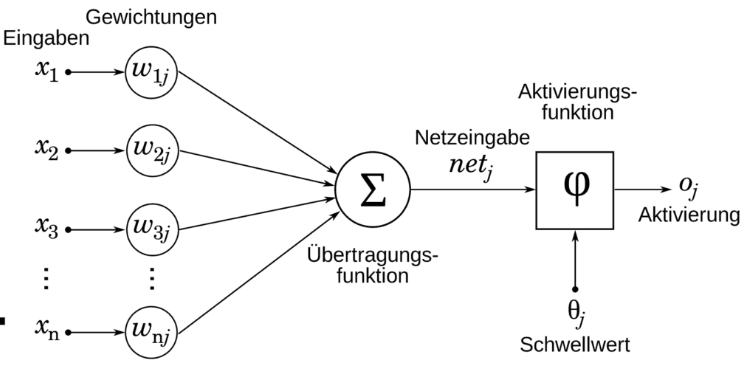
\includegraphics[height=5cm]{images/neuron2.png}
	\caption{Aufbau eines Neurons \cite{nndatasolutbasic}}
	\label{fig:neuron}
\end{figure}

Neuronen kommunizieren in dem sie kurze elektrische Impulse über Synapsen versenden, bzw. empfangen.
Erhält ein Neuron eine ausreichende Anzahl an Signalen innerhalb weniger Millisekunden, so feuert dies eigene Signale weiter.
Die einzelnen Neuronen sind in einem Netzwerk mit Milliarden von anderen Neuronen verbunden, in dem sie in fortlaufenden Layern eingegliederd sind (siehe Abbildung \ref{fig:biological_nn}) \cite{geron2019hands-on}. 
\begin{figure}[htbp]
	\centering
		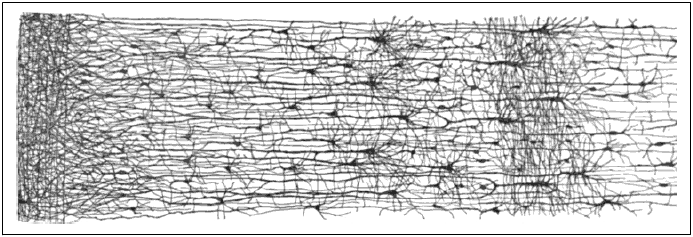
\includegraphics[height=4cm]{images/biological_nn.png}
	\caption{Multiple Layer in einem biologischen neuronalen Netzwerk \cite{geron2019hands-on}}
	\label{fig:biological_nn}
\end{figure}
 
Künstliche neuronale Netzwerke spiegeln das Verhalten des menschlichen Gehirns wieder und ermöglichen es Computerprogrammen selbständig Muster zu erkennen und allgemeine Probleme zu lösen \cite{nnibm}. 
%\begin{wrapfigure}{l}{0.5\textwidth}
%	\centering
%		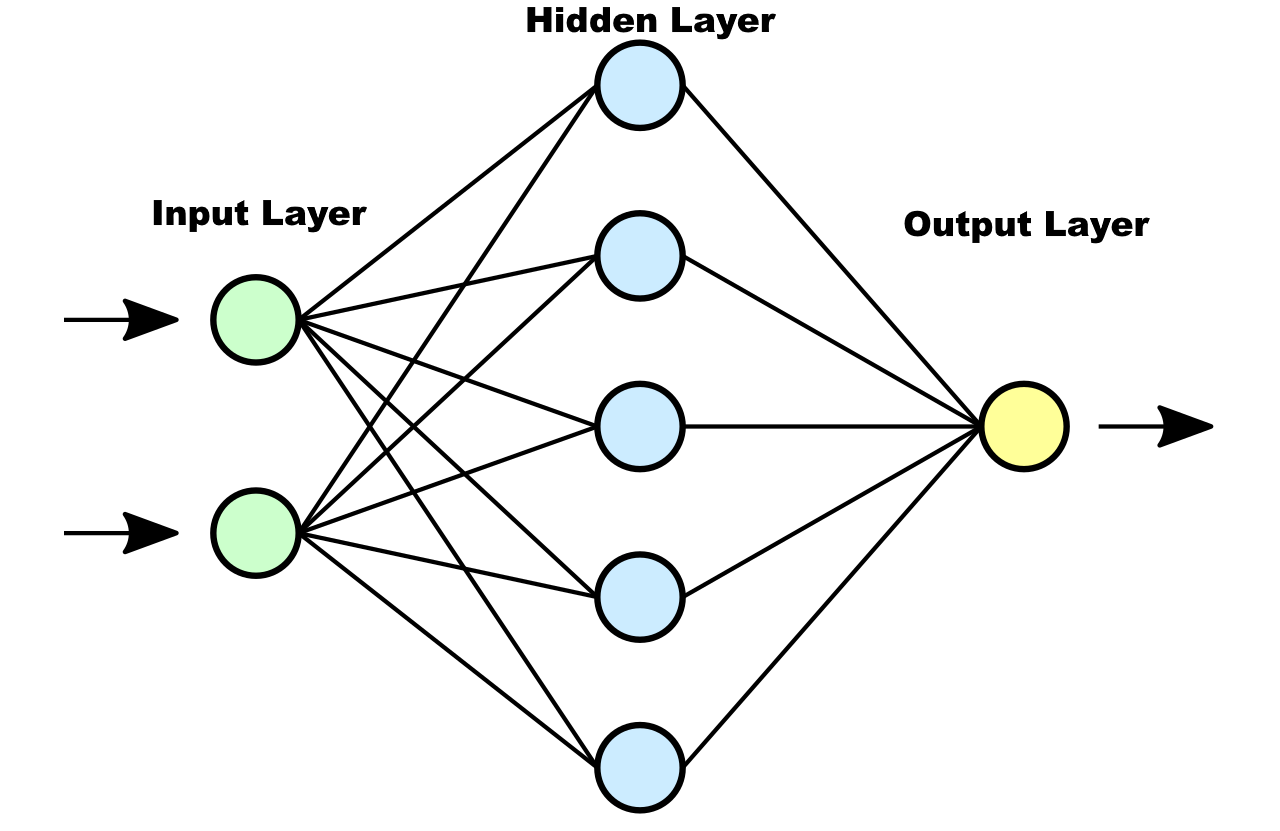
\includegraphics[height=5cm]{images/neural_network.png}
%	\caption{Einfache Veranschaulichung eines neuronalen Netzwerkes \cite{nnwiki}}
%	\label{fig:neuronal_network}
%\end{wrapfigure}
Künstliche neuronale Netzwerke können verschiedene Datenquellen wie Geräusche, Bilder, Texte, Tabellen oder Zeitreihen interpretieren, woraus sie Informationen extrahieren und Muster erkennen um später auf unbekannte Daten Vorhersagen treffen zu können.
Grundsätzlich weisen künstliche neuronale Netzwerke die Strukturen gerichteter Graphen auf, können aber je nach komplexität unterschiedlich aufgebaut sein \cite{nndatasolutbasic}. 

Angelehnt an die Struktur eines biologischen neuronalen Netzwerkes besteht ein künstliches neuronales Netzwerk ebenfalls aus Neuronen, welche in Layern (Schichten) angeordnet sind.
Ein solches Netzwerk besteht aus einem Input-Layer, einem (oder mehreren) Hidden-Layer und einem Output-Layer (veranschaulicht in Abbildung ~\ref{fig:neural_network}), wobei jeder dieser Layer eine Vielzahl an Neuronen beinhaltet.
Desto komplexer das zu lösende Problem ist, umso mehr Layer werden benötigt \cite{nnionos}. 
Der Input-Layer nimmt die eingegebenen Daten entgegen, verarbeitet und gewichtet diese, bevor sie an den Hidden-Layer weiter gegeben wird \cite{nndatasolutbasic}.
Der Hidden-Layer befindet sich zwischen Input und Output-Layer \cite{nndatasolutbasic} und kann aus einem oder mehreren Layern bestehen und ist der Layer, in dem die meisten Berechnungen stattfinden \cite{nnmedium}.
Auch in diesem Layer finden wieder Gewichtungen statt.
Sind mehere Layer im Hidden-Layer vorhanden, so geschieht das Gewichten pro Layer \cite{nndatasolutbasic}. 
Die Ausgabewerte des letzten Hidden-Layers werden dem Output-Layer als Eingabewerte übergeben \cite{nnmedium}.
Der Output-Layer ist die letzte Schicht und beinhaltet die Entscheidung oder Vorhersagung des neuronalen Netzwerkes \cite{nndatasolutbasic}.
\begin{figure}[htbp]
	\centering
		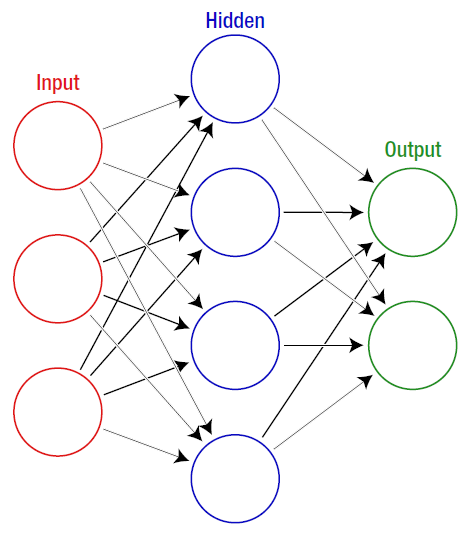
\includegraphics[height=6cm]{images/neural_network2.png}
	\caption{Einfache Veranschaulichung eines neuronalen Netzwerkes \cite{practicalml}}
	\label{fig:neural_network}
\end{figure}
Eine angemessene Anzahl an Neuronen und eine passende Ativierungsfunktion sollte je nach Aufgabe gewählt werden. 
In den Neuronen werden Berechnungen getätigt \cite{nnpathmind} und jedes Neuron hat ein zugeordnetes Gewicht, wodurch sie unterschiedliche Wichtigkeiten erhalten \cite{nnionos}.
%In biologischen neuronalen Netzwerken agieren Synapsen wie Gewichte über die eingehenden Impulse \cite{GURESEN2011426}.
Im biologischen Kontext können Gewichte mit Synapsen verglichen werden \cite{GURESEN2011426}.
Kombiniert mit einer Übertragungsfunktion entscheidet das Gewicht über den Input eines Neurons \cite{nnionos}.
Bei den künstlichen neuronalen Netzwerken kombiniert ein Neuron die Eingangssignale mit zugeordneten Gewichten, welche die Bedeutung des Signals schwächen oder verstärken. 
Nach dem Aufsummieren wird das Ergebnis durch eine Aktivierungsfunktion gegeben um zu berechnen ob, und mit welchem Ausmaß das Ausgangssignal weitergesendet wird.
Das Neuron wird als aktiviert bezeichnet, wenn es ein Ausgangssignal versendet \cite{nnpathmind}. 

\subsection{Arten von neuronalen Netzwerken}
Es gibt viele verschiedene Arten von küntlichen neuronalen Netzwerken und es werden nun ein paar davon etwas näher erläutert.

\subsubsection{Preceptron}
Preceptron ist ein neuronales Netzwerk mit nur einem Layer \cite{preceptrontowards}, welches im Bereich von supervised Learning Anwendung findet \cite{preceptronsimplilearn}.
Es ist ein linearer oder binärer Klassifizierer und wird verwendet um Daten in zwei Gruppen zu klassifizieren \cite{preceptrontowards}.
Ein Preceptron funktioniert folgendermaßen:
\begin{enumerate}
	\item Alle Eingangssignale werden mit ihren Gewichten multipliziert
	\item Nach dem multiplizieren wird alles Aufsummiert
	\item Abschließend wird eine Aktivierungsfunktion angewendet, welche den Wert auf den gewünschten Wert, wie z.B. (0,1) mapt. \cite{preceptrontowards}
\end{enumerate}

\subsubsection{Feed forward neuronale Netzwerke}
Ein Preceptron ist eine From von Feed forward neuronalen Netzwerken, welche die einfachste Form von neuronalen Netzwerken sind \cite{ffnndeepai}.
Informationen werden nur in eine Richtung, von Input-Layer über Hidden-Layer zum Ausgangs-Layer verarbeitet.
Abbildung ~\ref{fig:neural_network} veranschaulicht ein feed forward neuronales Netzwerk und die funktionsweise ist gleich wie bei Preceptrons.
Wenn es viele Layer zwischen dem Input und Output-Layer gibt, so wird es auch als deep feed forward neural network bezeichnet. \cite{ffnnat}

\subsubsection{Convolutional neuronale Netzwerke}
Convolutional neural networks sind eines der beliebtesten deep neural networks \cite{cnnieee}.
Der Name kommt von der mathematischen Linearfunktion convolution, welche auf Matrixen angewandt wird \cite{cnnieee}.
CNNs sind effizient mit 2D und 3D Eingabedaten und werden unter anderem für Objektdetektion bei Bildern verwendet \cite{nndatasolutbasic}.
Die Architektur ist unterschiedlich zu klassischen neuronalen Netzwerken, mehr dazu in Kapitel \ref{cnn}.

\subsubsection{Recurrent neuronale Netzwerke}
Wenn es um sequentielle oder zeitliche Daten geht so können feed forward neuronale Netzwerke nicht verwendet werden.
Es wird ein Mechanismus benötigt um historische Daten zu speichern und desshalb wurden Recurrent neuronale Netzwerke entwickelt.
In klassischen feed forward neuronalen Netzwerken sind alle Datenpunkte unabhängig von einander, was mit sequentiellen Daten, welche von vorherigen Daten abhängig sind, nicht funktioniert \cite{recurrentnnmastery}. 
Recurrent neuronale Netzwerke haben ein Konzept mit dem sie Informationen über vorherige Daten speichern können.
Dieses Konzept wird Memory genannt. \cite{recurrentibm}

\subsection{Training bei Neuronalen Netzwerken}
Ein Vorteil von künstlichen neuronalen Netzwerken ist, dass beim Erstellen nicht alle Parameter spezifiziert werden müssen, da der Algorithmus anhand von Beispielen von selbst lernt \cite{deeplearningnn}.
Neuronale Netzwerke können grundsätzlich für jedes komplexe Problem verwendet werden, bei dem es sich um funktionale Beziehungen handelt. 
Es ist hierbei nicht notwendig die Art der Beziehung zu kennen, da das neuronale Netzwerk durch das Beobachten und iterativem anpassen der Parameter lernt \cite{neuralnettraining}.

Um zu verstehen wie gut ein solches Netzwerk für eine bestimmte Aufgabe performt kann die Verlustfunktion verwendet werden.
Zu Beginn wird ein neuronales Netzwerk mit zufälligen Gewichten versehen, was in einem schlecht performenden neuronalem Netzwerk resultiert. 
Das Ziel ist es die hohe Verlustfunktion durch das Trainieren des neuronalen Netzwerkes in eine niedrige zu verwandeln  \cite{nntowards}.
Eine Methode für das fine-tuning von neuronalen Netzwerken ist Backpropagation.
Dabei handelt es sich um eine Methode zur Anpassung der Gewichte eines neuronalen Netzwerkes, welche als Grundlage die Fehlerquote der vorangegangenen Iterationen (bei neuronalen Netzwerken Epochen genannt) hernimmt. 
Durch das richtige adaptieren der Gewichte kann die Fehlerquote verringert und die Genauigkeit des Models erhöht werden \cite{backpropagationguru}. 
Gewichte verstärken oder schwächen die Signale der Neuronen und geben die Wichtigkeit eines bestimmten Bereiches der Daten an.
Ein Neuron kann ein bestimmtes Muster erkennen und die Bedeutung dieses Muster für das Gesamtkonstrukt entscheidet sich je nach Gewicht \cite{nnohv}.

\subsection{Anwendungsbeispiel eines neuronalen Netzwerks}
Um ein besseres Verständis für neuronale Netzwerke zu bekommen folgt nun ein Anwendungsbeispiel mit kleinen Codesnipets.
Ziel ist es ein neuronales Netzwerk aufzubauen, welches ein Bild einer handgeschriebenen Zahl richtig klassifizieren kann.
Hierfür wird der MNIST Datensatz \footnote[1]{MNIST Datensatz erhältlich unter http://yann.lecun.com/exdb/mnist/} verwendet, welcher 60000 28 mal 28 Pixel große Graustufenbilder von handgeschriebenen Zahlen von 0 bis 9 beinhaltet.
Um den MNIST Datensatz zu laden wird Tensorflow und Keras verwendet (siehe Listing \ref{lst:mnist}).
\begin{lstlisting}[frame=lines, caption=MNIST Datensatz in Python laden, captionpos=b, label = lst:mnist, language=Python, showstringspaces=false]
from tensorflow.keras.datasets import mnist
# load dataset
(trainX, trainy), (testX, testy) = mnist.load_data()
\end{lstlisting}
Die Bilder aus dem MNIST Datensatz sind in Abbildung ~\ref{fig:mnist_data} zu sehen.
\begin{figure}[htbp]
	\centering
		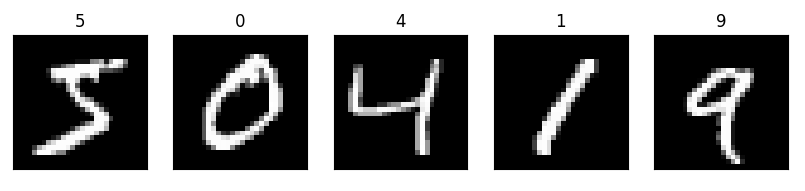
\includegraphics[height=3.5cm]{images/mnist_data.png}
	\caption{Beispielbilder aus dem MNIST Datensatz}
	\label{fig:mnist_data}
\end{figure}
Die Architektur des neuronalen Netzwerkes hat 784 (28 mal 28) Neuronen im Input-Layer. 
Somit kann jeder Pixel eines Bildes an ein Neuron als Eingabedaten übergeben werden.
Der Hidden-Layer beinhaltet 15 Neuronen, wobei die Anzahl hier variieren kann.
Abgeleitet von den vorhandenen Klassen (0 bis 9) ergeben sich sich 10 Neuronen im Output-Layer.
Um diese Architektur mithilfe von Keras und Tensorflow in Pyhton nachzubilden können die Codezeilen aus dem Listing \ref{lst:architecture_nn} verwendet werden.
\begin{lstlisting}[frame=lines, caption=Architektur des Neuronalen Netzwerkes, captionpos=b, label = lst:architecture_nn, language=Python, showstringspaces=false]
from keras.layers import Dense
from keras.models import Sequential
image_size = 784 # 28*28 Pixel
num_classes = 10 # Zahlen von 0 bis 9
model = Sequential()
model.add(Dense(units=15, activation='sigmoid', input_shape=(image_size,)))
model.add(Dense(units=num_classes, activation='softmax'))
model.summary()
\end{lstlisting}
Dense bedeuted dass es sich um ein vollständig verbundenes Netzwerk handelt, was bedeutet dass jedes Neuron des Input-Layers mit jedem Neuron aus dem nächsten Layer verbunden ist.
Dies ist in Abbildung  ~\ref{fig:mnist_neural_network} zu sehen, welche die Beschriebene Architektur des neuronalen Netzwerks veranschaulicht.
\begin{figure}[htbp]
	\centering
		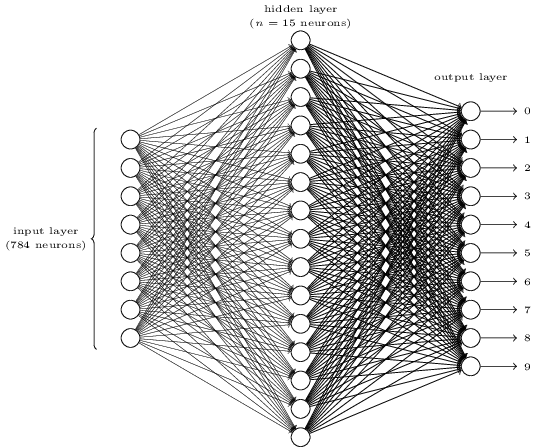
\includegraphics[height=9cm]{images/mnist_neural_network.png}
	\caption{Architektur des Neuronalen Netzwerks \cite{nnarchitecture}}
	\label{fig:mnist_neural_network}
\end{figure}
Vor dem Compilieren und Trainieren des neuronalen Netzwerkes werden die Testdaten noch modifiziert, was im kompletten Codebeispiel im Anhang \ref{lst:mnist_example} zu finden ist.
\begin{lstlisting}[frame=lines, caption=Model compilen und erlernen, captionpos=b, label = lst:model_compile_train, language=Python, showstringspaces=false]
model.compile(loss='categorical_crossentropy', optimizer='sgd',metrics=['acc']) 
history = model.fit(x_train, y_train, batch_size=128, epochs=5, verbose=False, validation_split=.1)
loss, accuracy  = model.evaluate(x_test, y_test, verbose=False)
\end{lstlisting}
Als Verlustfunktion wird hier die categorical crossentropy verwendet, da diese für Mehrklassenklassizierung, bei der ein Datensatz genau einer Klasse angehört, gut geeignet ist \cite{categoricalcrossentropy}.
Stochastic Gradient Descent gehören zu den einfachsten Optimierer, weshalb sie in diesem Besipiel für das Model gewählt wurden.
\begin{figure}
\center
\subfigure[5 Epochen]{\label{fig:5_epochs}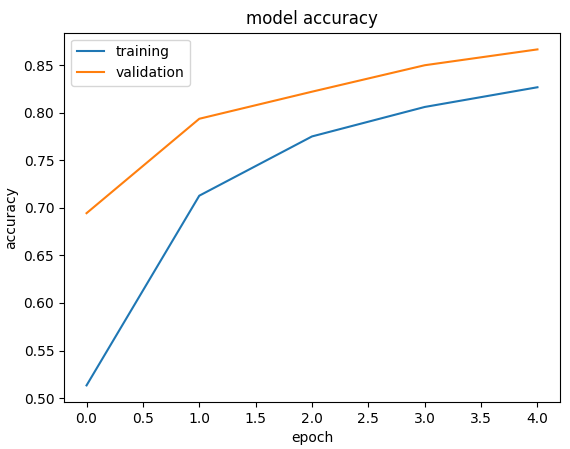
\includegraphics[width=70mm]{images/mnist_5_epochs.png}}
\subfigure[50 Epochen]{\label{fig:50_epoochs}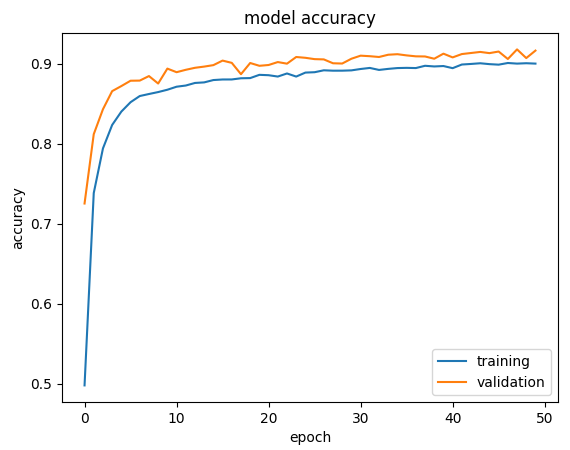
\includegraphics[width=70mm]{images/mnist_50_epochs.png}}
\caption{Vergleich 5 und 50 Epochen}
\label{fig:5_vs_50_epochs}
\end{figure}
Für das Trainieren des Algorithmus wurden zum Vergleich einmal 5 und einmal 50 Epochen ausgewählt.
Wie in Abbildung ~\ref{fig:5_vs_50_epochs} zu sehen ist erreicht das Model nach 5 Epochen eine Genauigkeit von etwas mehr als  80\%, während es nach 50 Epochen eine Genauigkeit von fast 90\% erreicht.
Die Architektur und der Aufbau des neuronalen Netzwerkes könnte noch deutlich verändert und optimiert werden, jedoch dient dieses Beispiel zum Verständis.


\chapter{Bildbezogenes Machine Learning}
\label{sec:imagerelatedml}
Die Digitalisierung und Automatisierung von Abläufen nimmt auf der ganzen Welt rasant zu.
Bilverarbeitung im Kontext von Computern und machine Learning bezieht sich darauf wichtige und bedeutende Informationen aus Bildern zu extrahieren.
Da Bilder mittels unstrukturierten Daten repräsentiert werden, ist es weitaus schwieriger diese im Gegensatz zu strukturierten Daten wie Tabellen zu interpretieren.
Je nach Anwendung gibt es unterschiedliche Methoden und Algorithmen, welche verwendet werden können.
Der große Bereich von Computer Vison, welcher zudem stetig wächst, wird bereits in verschiednen Bereichen wie Video Verarbeitung, Gesichtserkennung, Medizinisches Umfeld, Robotic Vision, Selbstfahrende Autos und vieles mehr eingesetzt \cite{autonomouscarsimageprocessing}.
Während Tesla bereits autonome und selbständig fahrende Autos verkauft, hat Apple Ende 2021 einen Techniker von Tesla angeheuert und plant 2024 selbstfahrende Autos auf den Markt zu bringen \cite{reutersapple}.
Bildverarbeitung und Bilderkennung spielen hierbei eine große Rolle, da Objekte wie Fahrspur, Ampel und andere Verkehrsteilnehmer richtig und zeitgerecht erkannt werden müssen \cite{autonomouscarsimageprocessing}.

Auch im medizinischen Bereich hat machine Learning einen großen Einfluss.
Neuronale Netzwerke, insbesondere deep learning Methoden wie Convolutional neural Networks (siehe Kapitel \ref{cnn}), werden bereits für medizinische Bildanalyse wie Bildsegmentierung, Klassifizierung und Problemvorhersagungen verwendet und unterstützden dabei medizinische Experten \cite{KE2019218}.
Durch das Analysieren von Röntgenbildern der Brust können mithilfe von machine Learning COVID-19 Patienten, mit einer Genauigkeit von 96.78\%, erkannt werden \cite{covidpaper}.

\section{Wie computer sehen}
\label{sec:howcomputersee}
Seit über 60 Jahren versuchen Wissenschaftler auf der ganzen Welt Maschinen beizubrignen, wie sie bedeutungsvolle Informationen aus visuellen Daten extrahieren können \cite{computervisioncnnhackernoon}.
Allgemein gilt Computer Vision als eines der komplexesten Gebiete im Bereich von künstlicher Intelligenz \cite{computerseestemera}.
Bereits im Jahre 1959 beschäftigten sich die Neurophysiologen David Hubel und Torsten Wiesel mit dem Thema Computer Vision, welches ein Teilbereich von künstlicher Intelligenz ist, und den Zweck verfolgt Systemen das erkennen von bedeutsamen Informationen aus Bildern oder Videos zu extrahieren \cite{computervisionibm,computervisioncnnhackernoon}.
Ihre Publikation "Receptive fields of single neurons in the cat's striate cortex"\cite{computervisioncat} gilt als eines der Papers, welches am meisten Einfluss auf die Thematik genommen hat \cite{computervisionibm,computervisioncnnhackernoon}.
Dabei beschreiben sie ihre Experimente, bei denen sie Elektroden and den primären Bereich des visuellen Kortex von anesthisierten Katzen angeschlossen haben, und diese dabei beobachtet haben, während den Versuchtieren verschiedene Bilder gezeigt wurden.
Durch einen glücklichen Zufall sind sie zur Erkenntniss gekommen, dass es sowohl einfache, als auch komplexe Neuronen im primären visuellen Kortex gibt, und dass visuelle Verarbeitung immer mit simplen Strukturen wie Kanten und Rändern beginnt.
Dieser Ansatz findet Anwendung bei convolutional neural networks und ist im Wesentlichen das Grundprinzip von deep Learning \cite{computervisioncnnhackernoon}. 
Bevor es tiefer in diese Materie geht, wird im folgenden Unterkapitel kurz definiert und veranschaulicht was ein Bild ist und wie ein Computer solch eines wahrnimmt.

\subsection{Was ist ein (digitales) Bild?}
Ein digitales Bild repräsentiert Bildinhalte mittles ganzen Zahlen \cite{digitalimagewiki}.
Es handelt sich dabei um eine digitale Repräsentation von etwas, das erstellt und kopiert werden kann und in elektronischer Form gespeichert wird \cite{digitalimagetechtarget}. 
Grundsätzlich wird bei digitalen Bildern zwischen zwei verschiedenen Arten unterschieden:
\begin{itemize}
	\item \textbf{Rastergrafiken}: die Informationen werden in gleichmäßiger Rasterung gespeichert \cite{digitalimagewiki}. Das Bild bestehr aus einer endlichen Anzahl an digitalen Bildelementen, welche auch als Pixel bekannt sind \cite{digitalimageenwiki} und welche in Reihen und Spalten angeordnet sind \cite{computerseesrealpython}. Die Anzahl der Pixel auf Reihe und Spalte ergeben die Auflösung eines Bildes. Ist ein Bild 200 Pixel breit und 400 Hoch, so hat es z.B. eine Auflösung von 200x400 Pixeln \cite{computerseesrealpython}.
	\item \textbf{Vektorgrafik}: die Informationen werden durch geometrische Objekte wie Punkte, Flächen oder Linien, definiert \cite{digitalimagewiki}.
\end{itemize}
Es ist auch möglich Raster und Vektorgrafiken zu kombinieren und daraus ein digitales Bild zu generieren \cite{digitalimageenwiki}.
Um digitale Bilder für Menschen sichtbar zu machen benötigt es geeignete Anzeigegeräte wie Projektoren oder Computerbildschirme \cite{digitalimagewiki}.
Farbige Bilder werden oft nach dem RGB-Modell repräsentiert.
RGB steht für \textbf{R}ed \textbf{G}reen und \textbf{B}lue und jeder Pixel beinhaltet einen Mix aus diesen Farben, welche in drei Zahlen repräsentiert werden.
In einem Graustufenbild beinhaltet ein Pixel nur eine Zahl, welche die Intensität oder den Anteil an Licht repräsentiert \cite{computerseesrealpython}. 
Ein Computer kann ein Bild nicht wie wir Menschen sehen, für Maschinen sind digitale Bilder nur Zahlen \cite{computerseesmedium}.
Durch das Analysieren der Anordnung der Zahlen ist es einem Computer möglich ein Bild zu interpretieren. 
Ein ausreichend große Menge an Daten gilt als große Schwierigkeit wenn es darum geht Computern das erkennen und klassifizieren zu erlernen. \cite{computerseestemera}
\begin{figure}[htbp]
	\centering
		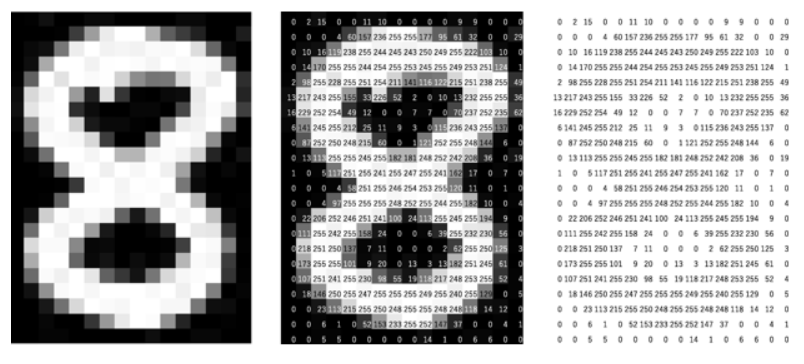
\includegraphics[height=6cm]{images/image_in_numbers.png}
	\caption{Repräsentation eines Bildes in Zahlen \cite{computerseesmedium}}
	\label{fig:image_in_numbers}
\end{figure}

In Abbildung \ref{fig:image_in_numbers} ist ein Graustufenbild von der Zahl 8 aus dem MNIST Datensatz abgebildet.
Hierbei ist ersichtlicht wie ein Computer dieses Graustufenbild anhand von Zahlen zwischen 0 und 255, welche die Intensität respräsentieren, auffasst.

\subsubsection{Dateiformate}
Digitale Bilder können in verschiedenen Dateiformaten gespeichert werden. 
In Tabelle \ref{tab:fileendings} sind einige davon beschrieben.
Bei Bildern spielt Komprimierung eine Rolle, da so die Dateigröße verringert werden kann.
Es gibt zwei verschiedene Arten von Komprimierung, Lossless und Lossy.
Bei der Lossless wird das Bild Komprimiert ohne dabei einen Qualitätsverlust zu erleiden \cite{imagefileformats}. 
Das Bild wird komprimiert abgespeichert, sobald darauf zugegriffen wird, werden jedoch alle benötigten Informationen wiederhergestellt und das ursprüngliche Bild ausgegeben \cite{practicalml}. 
Eine Lossy Komprimierung bedeuted hingegen dass Teilinformationen verloren gehen \cite{imagefileformats}.
Die Prorität bei dieser Komprimierung liegt dabei Speicherplatz zu sparen \cite{practicalml}. 
\begin{table*}[htbp]
	\centering
		\begin{tabular}{|c|c|c|m{20em}|}
		\hline
		\rowcolor[gray]{0.9}
		Dateiformat & Dateiendung & Komprimierung & Beschreibung \\
		\hline
		BITMAP & .bmp & keine & Bitmap wurde von Microsoft für Windows entwickelt. Es gibt bei diesem Dateiformat keine komprimierungm was jedoch in hohen Dateigrößen resultiert. \cite{imagefileformats} \\
		JPEG & .jpg .jpeg & Lossy & JPEG steht für Joint Potographic Experts Group und sind im Internet sehr verbreitet und ein beliebtes Dateiformat für Digitalkameras \cite{imagefileformats}. \\
		GIF & .gif & Lossless & GIF bedeuted Graphic Interface Format und bestizen tyischerweise sehr kleine Dateigrößen. Sie sind limitiert auf 256 Farben, können animiert werden und sind weit verbreitet im Web.  \cite{imagefileformats} \\
		PNG & .png & Lossless & PNG oder Portable Network Graphics wurde ursprünglich entwickelt um eine verbesserte Version des GIF Formates zu werden und dieses abzulösen. PNG Dateien können bis zu 16 Millionen Farben beinhalten.  \cite{imagefileformats} \\
		\hline	
		\end{tabular}
	\caption{verschiedene Dateiformate}
	\label{tab:fileendings}
\end{table*}

\section{Bilderkennung und Klassifizierung}
\label{sec:recognitionandclassification}
Um große Mengen an unstrukturierten Bilddaten effizient analysieren zu können, benötigt es fortschrittliche Techniken wie machine Learning \cite{imgclassificationviso}.
Bildklassifizierung, welche oft auch als Bilderkennung bezeichnet wird \cite{imgclassificationblog}, ist eines der Hauptprobleme im Bereich Computer Vision \cite{GAVALI201999}.
Die Aufgabe für Computer Vision hierbei ist es herauszufinden, was ein Bild beinhaltet und repräsentiert.
Es wird als die Aufgabe bezeichnet, welche Gruppen von Pixeln oder Vektoren innerhalb eines Bilder nach bestimmten Regeln kennzeichnet und kategorisiert.
Dabei wird die Bildklassifizierung in zwei Bereiche unterteilt, unsupervised und superviced.
Bei der unsupervised Klassifizierung handelt es sich um eine vollautomatische Methode, bei der keine Trainingsdaten benötigt werden.
Machine Learning Algorithmen werden verwendet um die Datensätze zu analysieren und zu clustern, indem sie ohne menschliches Eingreifen Muster erkennen.
Beim supervised Ansatz wird mittels bereits klassifizierten Datensätzen trainiert, um so dann neue und unbekannte Datensätze zu klassifizieren.
Applikationen zur Bildklassifizierung werden in Bereichen wie Medizinische Bildanalyse, Objekterkennung in Satelitenbildern, Ampelkontrollsystemen und vielen anderen Bereichen eingesetzt \cite{imgclassificationviso}.

\subsection{Herausforderungen bei machineller Bilderkennung}
In der folgenden Liste sind die Herausforderungen von maschineller Bilderkennung aufgezählt:
\begin{itemize}
	\item \textbf{Viewpoint variation}: Ein Objekt kann aus verschiednen Sichtpunkten und betrachtet werden.
	\item \textbf{Scale variation}: Ein Objekt der selben Klasse kann in unterschiedlichen Größen auftreten.
	\item \textbf{Deformation}: Ein Objekt kann verformt sein.
	\item \textbf{Occlusion}: Objekte können von anderen Objekten verdeckt sein, so dass nur wenige Pixel des Objektes sichtbar sind.
	\item \textbf{Illumination condiftions}: Der Einfluss von Beleuchtung kann auf Pixelebende einen großen Einfluss haben.
	\item \textbf{Background clutter}: Ein Objekt kann sehr ähnlich zum Umfeld erscheinen und somit darin schwer erkennbar werden.
	\item \textbf{Intra-class variation}: Die Klasse eines Objektes kann sehr breit gefächert sein. Es gibt verschiedene Arten davon, welche ein eigenes Aussehen besitzen \cite{deeplearningcomputervision}.
\end{itemize}
Beim Modellieren einer Bildklassifizierung gilt es darauf zu schauen, dass es gegenüber dem Kreuzprodukt all dieser Herausforderungen invariant ist, während es gleichzeitig die Empfindlichkeit gegenüber jeder einzelnen Variation beibehält \cite{deeplearningcomputervision}.
In Abbildung \ref{fig:challenges_computer_vision} sind die oben genannten Herausforderungen bildlich veranschaulicht.
\begin{figure}[htbp]
	\centering
		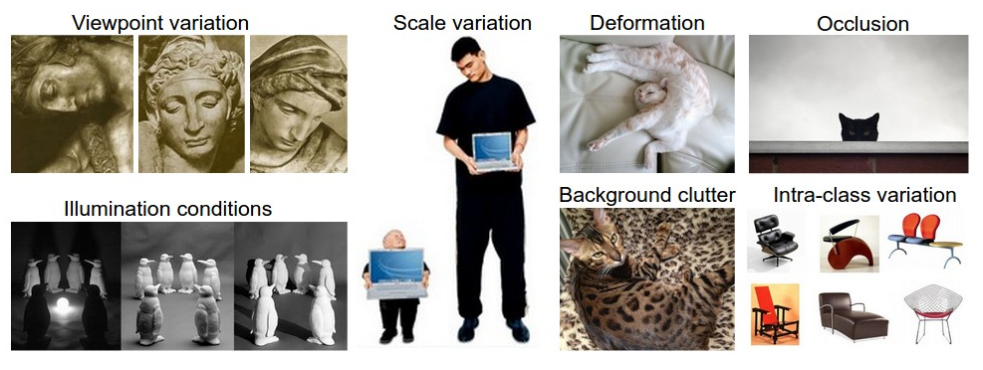
\includegraphics[height=5cm]{images/challenges_computer_vision.png}
	\caption{Beispiele für die Herausforderungen von maschineller Bilderkennung \cite{deeplearningcomputervision}}
	\label{fig:challenges_computer_vision}
\end{figure}

\section{Algorithmen für Bildähnlichkeitserkennung}
\label{sec:algorithmsimagesimilarity}

\subsection{SIFT}
\label{sift}
Scale Invariant Feature Transform, kurz SIFT, wurde erstmals 2004 von David Lowe in seinem Paper "Distinctive Image Features from Scale-Invariant Keypoints" \cite{siftlowe} veröffentlicht und ist eine Methode zur Überprüfung der Übereinstimmung von Bildern, welche auch zur Objekterkennung verwendet werden kann.
Es handelt sich dabei um eine Methode die Merkmale aus Bildern extrahiert, welche für einen zuverlässigen Abgleich zwischen verschiedenen Ansichten eines Objekts oder einer Szene sorgen \cite{siftlowe}. 
Die Extrahierung der Merkmale von Bildern erfolgt vor dem Abgleich unabhängig voneinander \cite{siftieee}.
Mit effizienten Algorithmen kann eine große Anzahl von Merkmalen aus typischen Bildern extrahiert werden.
Diese Merkmale sind gegenüber Skalierung, Rotation, und Beleuchtungsänderung invariant und weisen eine Robustheit gegenüber Verzerrung und dem Hinzufügen von Rauschen auf.  
Mittels SIFT Deskriptoren werden starke Interessenspunkte abgeglichen, um so ähnlichkeiten aufzuweisen \cite{siftlowe}. 

\subsubsection{Funktionsweise SIFT}
Folgende Schritte werden benötigt um Merkmale aus Bildern zu extrahieren:
\begin{enumerate}
	\item \textbf{Scale-space extrema detection}: in dieser Stufe, welche die erste Stufe von SIFT ist, werden alle Skalen und Koordinaten durchsucht \cite{siftieee}. Durch eine effiziente Implementierung der difference-of-Gaussian Funktion können potentiell interessante Punkte, welche invariant zu Skalierung und Orientierung sind, identifirziert werden \cite{siftlowe}.
	\item \textbf{Keypoint localization}: Einige gefundene Punkte sind nicht gut genug und können mittels Keypoint localization eliminiert werden. Sobald ein Schlüsselpunkt mittels Vergleich eines Pixels mit dessen Nachbarn gefunden wurde, folgt eine detaillierte Anpassung an die nahe gelegenen Daten in Bezug auf Lage, Skalierung und dem Verhältnis der Hauptkrümmungen. \cite{siftieee} Auf Grundlage von Stabilität werden die Schlüsselpunkte ausgewählt \cite{siftlowe}.
	\item \textbf{Orientation assignment}: Basierend auf lokalen Bildeigenschaften werden zu jedem Schlüsselpunkt konsistente Orientierungen zugewiesen, wodurch der Deskriptor des Schlüsselpunkts relativ zu dieser Aurichtung dargestellt werden kann \cite{siftieee}. 
	\item  \textbf{Keypoint descriptor}: Im ausgewählten Maßstab werden lokale Bildgradienten in der Region um jeden Schlüsselpunkt gemessen. Diese werden in eine Darstellung transformiert, welche ein hohes Maß an Formverzerrung und Beleuchtungsänderung zulässt. \cite{siftlowe} Es wird ein gewichtetes Richtungshistogram im Umkreis des Schlüsselpunktes erstellt und die Orientierung wird dann Anhand des höchsten Schlüsselpunktes ermittelt \cite{siftieee}.
\end{enumerate}
%https://ieeexplore-1ieee-1org-1tn53mdbb08d0.han.fh-campuswien.ac.at/stamp/stamp.jsp?tp=&arnumber=6754850
%https://www.cs.ubc.ca/~lowe/papers/ijcv04.pdf

\subsection{Convolutional Neuronal Networks}
\label{cnn}
Convolutional neuronal newtorks, die im Deutschen übersetzt als "Gefaltete Neuronale Netzwerke" bezeichnet werden, sind eine besondere From von künstlichen neuronalen Netzwerken, welche mehrere sogenannte Faltungsschichten beinhalten \cite{cnnbigdata}.
Seit den 1980er Jahren werden CNNs für visuelle Aufgaben verwendet \cite{10.1162/neco_a_00990}.
In den letzten zehn Jahren gab es durch convolutional neuronale Netzwerke bahnbrechende Ergebnisse in einer Vielzahl von Bereichen der Mustererkennung, von Bildverarbeitung bis zur Spracherkennung.
Einer der größten Vorteile von CNNs gegenüber regulären künstlichen neuronalen Netzwerken ist die reduzierte Anzahl der Parameter, wodurch es möglich ist größere Models, und somit komplexere Probleme zu lösen \cite{cnnieee}. 
Während bei primitiveren Methoden Filter von Hand entwickelt werden, so sind CNNs durch ausreichendem Training in der Lage Filter selbst zu erlernen \cite{cnntowards}.
Ein weiterer wichtiger Aspekt von CNNs ist es abstrakte Merkmale zu erkennen. 
Die Merkmale werden pro Schicht erkannt, so ist es z.B. möglich dass in der ersten Schicht einfache Kanten und Ränder erkannt werden, während in der zweiten Schicht schon einfache Formen identifiziert werden \cite{cnnieee}. 
Während sich sich die erste Schicht auf einfache Merkmale wie Farben und Kanten konzentriert, so sind tiefere Schichten in der Lage größere Elemente und Formen zu erkennen \cite{cnnibm}.
Das Netzwerk ist robust und gegenüber Verzerrungen oder optischen Veränderungen unempfindlich.
Es kann Bilder verarbeiten, welche in unterschiedlichen Perspektiven und Lichtverhältnissen aufgenommen wurden, und kann trotzdem typische Merkmale eines Bildes erkennen \cite{cnnbigdata}. 
Vom Grundprinzip ist ein CNN ein vollvernetztes neuronales Feed-Forward-Netzwerk was sich aus folgenden Schichten zusammensetzt:
\begin{itemize}
	\item Eingangs-Schicht,
	\item Convolutional-Schicht,
	\item Pooling-Schicht,
	\item vollständig verbundenen neuronalen Netzwerk und
	\item Ausgangs-Schicht .
\end{itemize}
Während auf Convolutional-Schicht weitere Convolutional-Schichten oder Pooling-Schichten folgen können, ist das vollständig verbundene neuronale Netzwerk die letzte Schicht vor der Ausgabe-Schicht \cite{cnnibm}.
In Abbildung \ref{fig:cnn_architecture} ist ein beispielhafter Aufbau eines CNNs dargestellt, bei dem es darum geht Bilder zu klassifizieren.
\begin{figure}[htbp]
	\centering
		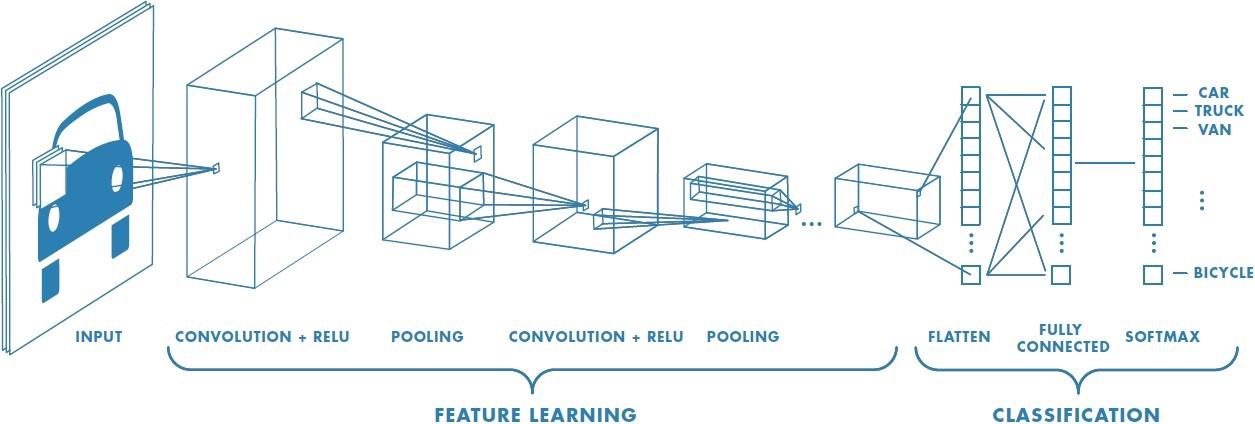
\includegraphics[height=5cm]{images/cnn.jpeg}
	\caption{Aufbau von CNN \cite{cnntowards}}
	\label{fig:cnn_architecture}
\end{figure}

\subsubsection{Convolutional-Schicht}
Die Convolutional-Schicht ist der zentrale Baustein eines CNN, in dem der Großteil der Berechnungen stattfindet \cite{cnnibm}.
Es  ist die eigentliche Faltungsebene und ist fähig aus den Daten Mermale wie Kanten, Linien oder bestimmte Formen zu erkennen und extrahieren \cite{cnnbigdata}.
Hauptanwendungen von CNNs sind Anwendungen mit Bildern, Sprache oder Audio Signalen \cite{cnnibm}.
\begin{figure}[htbp]
	\centering
		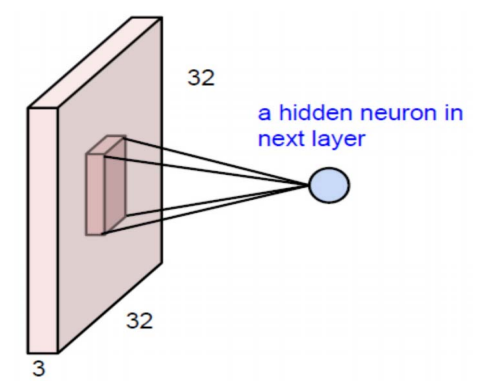
\includegraphics[height=4.5cm]{images/cnn_convolutional_example.png}
	\caption{Beispiel einer Convolution \cite{cnnieee}}
	\label{fig:convolution_example}
\end{figure}
%\begin{wrapfigure}{l}{0.4\textwidth}
%	\centering
%		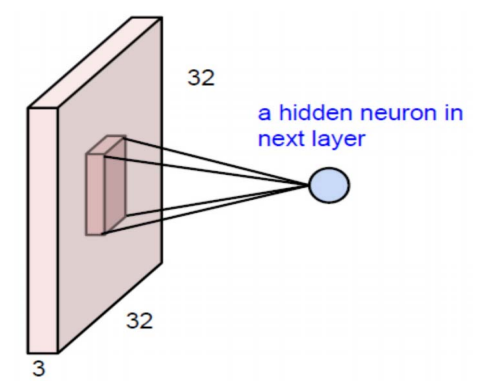
\includegraphics[height=4.5cm]{images/cnn_convolutional_example.png}
%	\caption{Beispiel einer Convolution \cite{cnnieee}}
%	\label{fig:convolution_example}
%\end{wrapfigure}
%\begin{wrapfigure}{r}{0.55\textwidth}
%	\centering
%		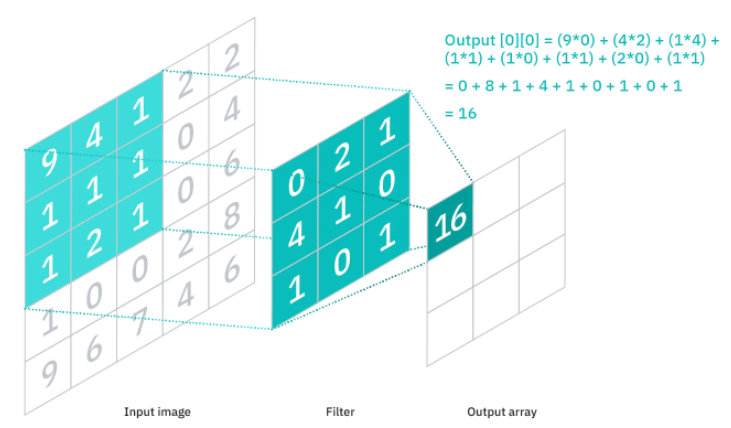
\includegraphics[height=5cm]{images/cnn_filter.png}
%	\caption{CNN Filter \cite{cnnibm}}
%	\label{fig:cnn_filter}
%\end{wrapfigure}

Um den Vergleich zu einem vollständig vernetztes neuronales Netzwerk, welches Pixel als Eingabe nimmt, folgt ein Beispiel.
Angenommen es handelt sich z.B. um ein 32 Pixel breites und hoches Bild, so werden hierfür bereits 32x32x3 (=3072) gewichtete Verbindungen benötigt.
32 für jeweils Breite und Höhe und dann noch jeweils 3 Kanäle für RGB.
Wird ein einzelnes Neuron im Hidden-Layer hinzugefügt so werden weitere 32x32x3 gewichtete Verbindungen benötigt.
Für eine aussagekräfitge Bilderkennung werden zwei Neuronen im Hidden-Layer nicht ausreichen, und somit steigt die Anzahl der gewichteten Verbindungen pro Neuron weiter an.
Um effizienter als normale vollständig vernetzte neuronale Netzwerke zu sein, betrachten CNNs anstelle des gesamten Bildes nur lokale Regionen davon. 
Wie in Abbildung \ref{fig:convolution_example} zusehen ist, bekommt der nächste Layer nur den dazugehörigen Teil von dem davorigen Layer, was in diesem Beispiel eine Verbindung zu einem 5x5 Neuron sein könnte.
Dadurch wird die Anzahl der benötigten gewichteten Verbindugen reduziert, da sich das CNN nur auf einen Teilbereich der Eingabedaten konzentriert.
Um die Anazhl der gewichteten Verbindungen weiter zu verringern können lokale gewichtete Verbindungen für die gesamten Neuronen des nächsten Layers beibehalten werden \cite{cnnieee}. 
\begin{figure}[htbp]
	\centering
		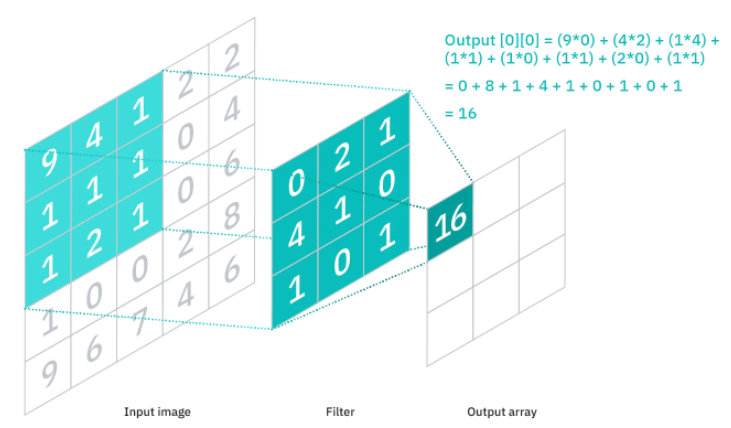
\includegraphics[height=5cm]{images/cnn_filter.png}
	\caption{CNN Filter \cite{cnnibm}}
	\label{fig:cnn_filter}
\end{figure}
Ein weiterer ähnlicher Ansatz ist ein Einfügen eines Fensters (z.B.5x5x3) \cite{cnnieee}, welches auch Kernel oder Filter genannt wird \cite{cnntowards} und welches über die Eingangsneuronen geschoben wird, und somit die dazugehörige Ausgabe an den dazugehörigen Platz verbindet \cite{cnnieee}.
Dieser Filter oder auch Feature-Detektor ist ein zweidimensionales Array bestehend aus Gewichten, welche Teile des Bildes repräsentieren.
Eine typische Größe dafür ist eine 3x3 Matrix, diese kann jedoch variieren.
Der Feature-Detektor wird dann auf einen Bereich der Eingabedaten angewandt, in dem das Kreuzprodukt zwischen den Eingabepixeln und dem Filter berechnet werden (siehe Abbildung \ref{fig:cnn_filter}).
Dieser Bereich wird auch als Receptive Field bezeichnet.
Das Ergebnis des Kreuzproduktes wird in ein Ausgabearray gespeichert und anschließend wechselt der Filter in Schritten (englisch: stride) und wiederholt den Vorgang bis der Filter über das ganze Bild angewandt wurde. 
Das endgültige Ergebnis aus der Reihe der Kreuzprodukte wird als Feature Map, Activation Map oder Convolved Feature bezeichnet \cite{cnnibm}. 

Strides geben an um wieviele Pixel sich der Filter weiter bewegt.
Standardmäßig wird ein Stride von 1 verwendet, wie auch in Abbildung \ref{fig:cnn_stride} dargestellt \cite{cnntowards}. 
Ein Stride von mehr als 1 verringert das Ausgabearray, wird in der Praxis jedoch eher selten angewandt \cite{cnncs231}.
\begin{figure}[htbp]
	\centering
		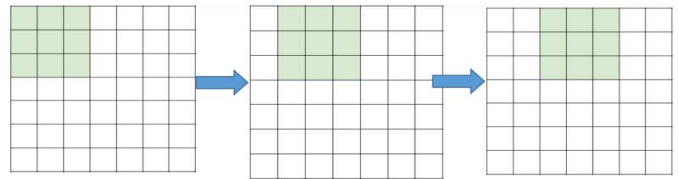
\includegraphics[height=3cm]{images/cnn_filter_moving2.png}
	\caption{Stride \cite{cnnieee}}
	\label{fig:cnn_stride}
\end{figure}
Während sich der Filter über das Bild bewegt, sind seine Gewichte fixiert, diese können sich jedoch während dem Training anpassen \cite{cnnibm}.
Einer der Nachteile des convolution Schrittes ist der Verlust von Informationen am Rande eines Bildes.
Da Informationen nur aufgenommen werden, wenn der Filter sich darüber bewegt haben sie nie die Chance gesehen zu werden.
Eine einfache Lösung dafür ist das sogenannte Zero-Padding \cite{cnnieee}. 
Padding ist der Prozess, bei dem der Eingangsmatrix symetrisch Nullen hinzugefügt werden \cite{cnntowards}.
Zero-padding wird in der Regel verwendet, wenn die Filter nicht zur Größe des Bildes passen, da mit Padding die Größe der Ausgangsmatrix verändert werden kann \cite{cnnibm}. 
Es gibt verschiedene Arten von Padding:
\begin{itemize}
	\item Valid padding: wird auch als no padding bezeichnet. Hierbei findet kein Padding statt und Informationen können verloren gehen, wenn die Größe von Filter und Eingangsdaten nicht übereinstimmt \cite{cnnibm}. 
	\item Same padding: durch Anwenden von same padding wird sichergestellt, dass die Größe der Ausgangsschicht gleich der Eingangsschicht ist \cite{cnnibm}.
\end{itemize}
Die Anzahl der Filter haben Einfluss auf die Tiefe der Ausgabe.
Drei Filter würden Beispielsweise drei verschiedene Feature Maps generieren und somit eine tiefe von drei ergeben \cite{cnnibm}. 
Nach jeder Faltungsoperation wendet ein CNN eine Nichtlinearitätsfunktion an \cite{cnnglassbox} um Nichtliniearität in das Model einzuführen \cite{cnnibm}.
Dies ist eine nichtlineare Gleichung, die es dem CNN ermöglicht, insgesamt kompliziertere Muster zu lernen.
Eine beliete Nichtlinearität ist Rectified Linear Unit Transformation (ReLu) \cite{cnnglassbox}. 
Letztendlich wandelt die Faltungsschicht das Bild in numerische Werte um, so dass das neuronale Netz relevante Muster interpretieren und extrahieren kann. 
Diese Methode bietet den Vorteil, dass aufgrund der Filter das Erkennen von Merkmalen unabhängig von der Position im Bild stattfinden kann \cite{cnnieee}. 

\subsubsection{Pooling-Schicht}
Die Pooling-Schicht wird auch Subsampling \cite{cnnbigdata} oder Downsampling Schicht genannt und der Hauptgedanke von pooling ist down-sampling um Komplexität für nachfolgende Schichten zu reduzieren \cite{cnnieee}.
Es werden dabei überflüssige Informationen verworfen und die Datenmenge wird verringert, wodurch sich die Berechnungsgeschwindigkeit erhöht \cite{cnnbigdata}.
Im Bereich der Bildverarbeitung kann Pooling auch als Verringern der Auflösung angesehen werden \cite{cnnieee}.
Die Berechnungen wären deutlich aufwendiger, würde man die Pooling-Schicht weglassen, und somit die Convolution Schicht direkt mit dem vollständig verbundenen neuronalen Netzwerk verbinden \cite{cnntowards}.
Ähnlich wie bei der Convolution-Schicht wird bei der Pooling-Schicht ein Filter über die Eingabedaten geschoben, jedoch hat dieser Filter keine Gewichte.
Stattdessen wird eine Aggregationsfunktion auf die Werte innerhalb des rezeptiven Feldes angewandt und somit die Ausgangfmatrix ausgefüllt \cite{cnnibm}. 
Es gibt verschiedene Arten von Pooling:
\begin{itemize}
	\item Max pooling: ist eines der weitverbreitesten Pooling Methoden \cite{cnnieee}. Während sich der Filter über den Eingabedatensatz bewegt, wird der Pixel mit dem größten Wert genommen und an das Ausgabearray gegeben \cite{cnnibm}.  Max Pooling wirkt auch als Rauschunterdrückung \cite{cnntowards}.
	\item Average pooling: Während sich der Filter über den Eingabedatensatz beweget, wird ein Mittelwert innerhalb des receptiven Feldes ermittelt und an das Ausgabearray übergeben \cite{cnnibm}.
\end{itemize}
\begin{figure}[htbp]
	\centering
		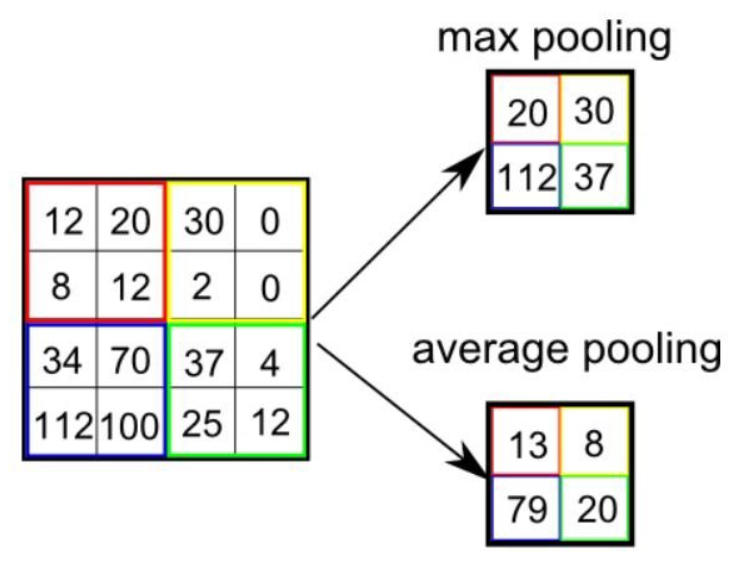
\includegraphics[height=4cm]{images/pooling.png}
	\caption{Max und Average Pooling \cite{cnntowards}}
	\label{fig:pooling}
\end{figure}

\subsubsection{Vollständig verbundenes neuronales Netzwerk}
Das vollständig verbundene neuronale Netzwerk folgt auf die Abfolgen von Convolutional- und Polling Schicht und bildet den Abschluss des convolutional neuronalen Netzwerk \cite{cnnbigdata}.
Der Aufbau des vollständig verbundenen neuronalen Netzwerk ähnelt der Art und Weise, wie die Neuronen in einem herkömmlichen neuronalen Netz angeordnet sind.
Jedes Neuron ist vollständig mit den Neuronen aus der vorherigen, und auch der nächsten Schicht verbunden \cite{cnnieee}.
Abhängig von den Klassen und Objekten, welche das neuronale Netzwerk bestimmen soll, werden die Anzahl der Neuronen bestimmt \cite{cnnbigdata}.
Der größte Nachteil der voll vernetzten Schicht ist es, dass es viele Parameter enthält, welche komplexe Berechnungen benötigen.
Um die Anzahl der Neuronen und Verbindungen zu verringern kann die Droput-Technik verwendet werden \cite{cnnieee}.
Über mehrere Epochen hinweg ist das Model in der Lage, zwischen dominierenden und bestimmten niederschwelligen Merkmalen in Bildern zu unterscheiden und diese mit Hilfe von Softmax zu klassifizieren \cite{cnntowards}.

%https://ieeexplore-1ieee-1org-1tn53mdbb0c2d.han.fh-campuswien.ac.at/stamp/stamp.jsp?tp=&arnumber=8308186
%https://towardsdatascience.com/a-comprehensive-guide-to-convolutional-neural-networks-the-eli5-way-3bd2b1164a53
%https://cs231n.github.io/convolutional-networks/
%https://www.bigdata-insider.de/was-ist-ein-convolutional-neural-network-a-801246/
%https://towardsdatascience.com/covolutional-neural-network-cb0883dd6529#:~:text=Examples%20of%20CNN%20in%20computer,i.e%2C%20weights%2C%20biases%20etc.

\subsection{Siamese Networks}
\label{siamesenetworks}
Im Bereich von Deep learning sind neuronale Netzwerke für fast jede Aufgabe geeignet, um jedoch gute Ergebnisse liefern zu können, sind diese auf ausreichend Daten angewiesen.
Traditionell werden sie verwendet um verschiedene Klassen vorherzusagen, wenn jedoch eine neue Klasse hinzukommt, so muss das neuronale Netzwerk aktualisert und erneut trainiert werden.
Zusätzlich sind meist nur wenige Daten für   bestimmte Probleme wie z.B. Gesichtserkennung oder Unterschriftenprüfung verfügbar.
Um diese Art von Problemen zu lösen wurden Siamesische Netzwerke entwickelt, welche eine neue Architekturart von neuronalen Netzwerken sind \cite{siamesetowards}. 
Erstmals wurden diese Netzwerke 1990 von Bromley und LeCun zum Zweck der Unterschriftenverifikation entwickelt \cite{siameseieee}.
Da Siamesische Netzwerke nur wenige Daten benötigen, wurden diese über die letzten Jahre immer beliebter.
Meist werden sie verwendet um Ähnlichkeiten in den Eingabedaten zu vergleichen \cite{siamesetowards}.

\subsubsection{Architektur}
Ein simaesischen Netzwerk (auch twin network genannt) hat seinen Namen von siamesischen Zwilligen, welche Zwillige sind, die phyiskalisch miteinander verbunden sind \cite{siamesepyimage}.
Es besteht aus zwei oder mehreren sogenannten Teil- oder Zwilligsnetzwerken, welche unterschiedliche Eingaben akzeptieren und identisch sind \cite{siameseieee, siamesetowards}.
Identisch bedeuted in diesem Fall dass die Teilnetzwerke die gleiche Konfiguration mit denselben Parametern und Gewichten besitzen.
Wenn Parameter aktualisiert werden, so werden diese gespiegelt in allen Teilnetzwerken ebenfalls aktualisiert \cite{siamesetowards}.
Eine Beispielarchitektur für ein siamesischen Netzwerk ist Abbildung \ref{fig:siamese_network} zu sehen.
\begin{figure}[htbp]
	\centering
		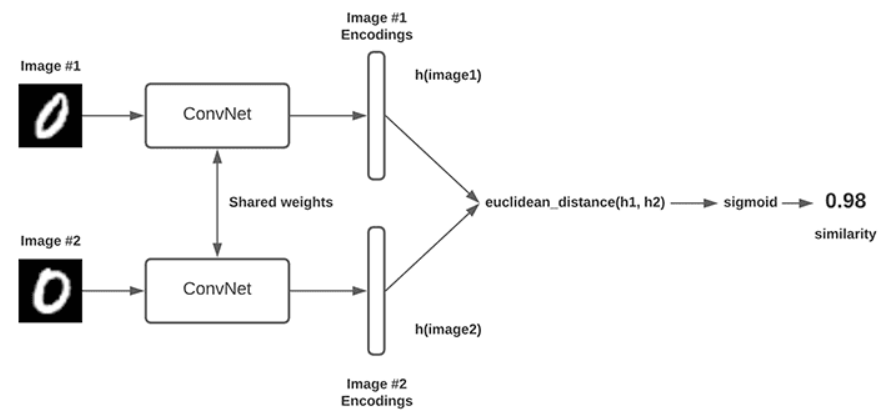
\includegraphics[height=7cm]{images/siamese_network.png}
	\caption{Beispielarchitektur Siamesisches Netzwerk \cite{siamesepyimage}}
	\label{fig:siamese_network}
\end{figure}
In diesem Fall werden zwei Bilder von handgeschriebenen Zahlen in zwei identische CNNs gegeben und anschließend wird die Euklidische Distanz berechnet.
Am Ende wird in die Sigmoid Aktivierungsfunktion angewandt, um anhand eines Ergebnises zwischen 0 und 1 die Ähnlichkeit auszudrücken.

% https://www.cs.cmu.edu/~rsalakhu/papers/oneshot1.pdf                    https://www.semanticscholar.org/paper/Siamese-Neural-Networks-for-One-Shot-Image-Koch/f216444d4f2959b4520c61d20003fa30a199670a
% https://towardsdatascience.com/a-friendly-introduction-to-siamese-networks-85ab17522942

\chapter{Prototyp zur Bildähnlichkeitserkennung von Markenlogos}
\label{chap:prototype}
In diesem Kapitel wird der Versuch beschrieben, einen Prototypen zu entwickeln, welcher zwei Eingabedaten entgegen nimmt und deren Ähnlichkeit ermitteln kann.
Es wird einerseits ein Versuch mittels \textbf{SIFT} und andererseits en Versuch mit einem \textbf{Siamesischem Netzwerk} beschrieben.

\section{Daten}
\label{sec:data}
Wie in der Einleitung bereits erwähnt beschäftigt sich das österreichische Patentamt viel mit Markenlogos und deren Ähnlickeit.
Da diese Masterarbeit in Zusammenarbeit mit dem östereichischen Patentamt entwickelt wird, haben sie mir dankenswerterweise ihre Logodaten zur Verfügung gestellt.
Diese Daten enthalten 210630 Bilder, welche in 213 Ordner unterteilt sind und was insgesamt 13.4 GB an Daten ausmacht.
Die Ordnerstruktur ist nach Anmeldungsjahr der Markenlogos gegliedert (siehe Abbildung \ref{fig:data_folderstructure}).
\begin{figure}[htbp]
	\centering
		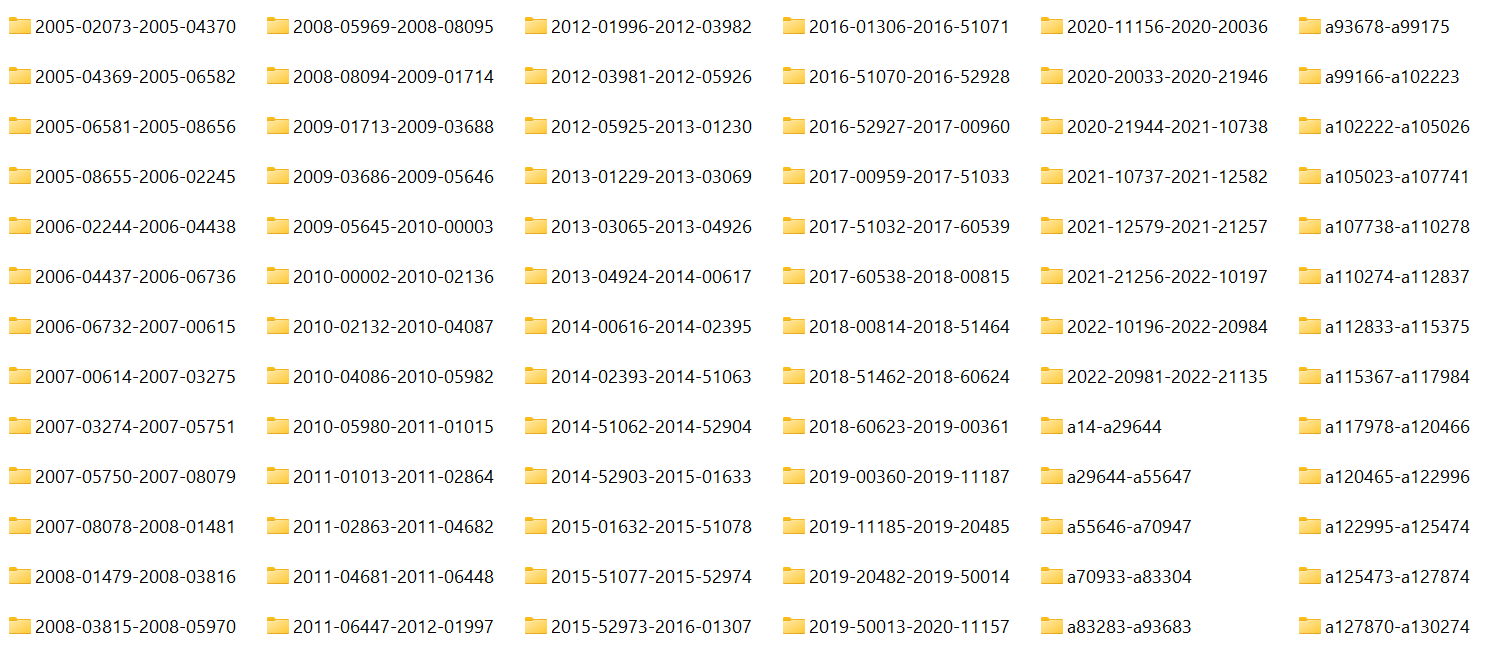
\includegraphics[height=7cm]{images/data_folderstructure.png}
	\caption{Ordnerstruktur der Markenlogos}
	\label{fig:data_folderstructure}
\end{figure}
Die Bilder in den jeweiligen Ordnern sind mittels Anmeldungsjahr und einer fortlaufenden Nummer beschrieben (siehe Abbildung \ref{fig:data_inside_folder}).
\begin{figure}[htbp]
	\centering
		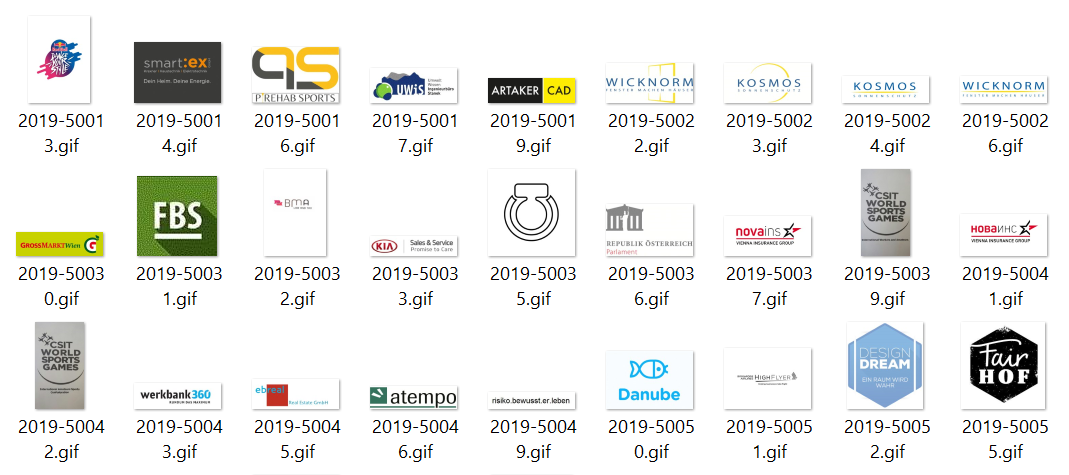
\includegraphics[height=7cm]{images/data_inside_folder.png}
	\caption{Datenstruktur in den Ordnern}
	\label{fig:data_inside_folder}
\end{figure}
\newpage
Um die Daten etwas besser verstehen zu können habe ich mir zwei Hilfsfunktionen geschrieben.
Mittels folgender Funktion (Listing \ref{lst:smallest_biggest}) wird das kleinste und größte Bild ermittelt.
\begin{lstlisting}[frame=lines, caption=Hilfsfunktion zur Ermittlung des kleinsten und größten Bildes, captionpos=b, label = lst:smallest_biggest, language=Python, showstringspaces=false]
def get_smallest_and_largest_image(filenames):
	all_images = []
	for filename in filenames:
		img = PILImage.open(filename, 'r')
		all_images.append([img.filename, img.size])
	sort = sorted(all_images, key=lambda x:x[1])
	return [sort[0],sort[-1]]
\end{lstlisting}
Die Funktion nimmt eine Liste von Dateinamen entgegen und ermittlet zuerst von jedem Bild die Größe und anschließend wird die Liste dann nach der Größe sortiert.
Somit befindet sich das kleinste Bild an erster und das größte an letzter Stelle, welche am Ende der Funktion zurückgegeben werden.
Das Ergebnis is in Abbildung \ref{fig:data_smallest_largest} zu sehen.
\begin{figure}[htbp]
	\centering
		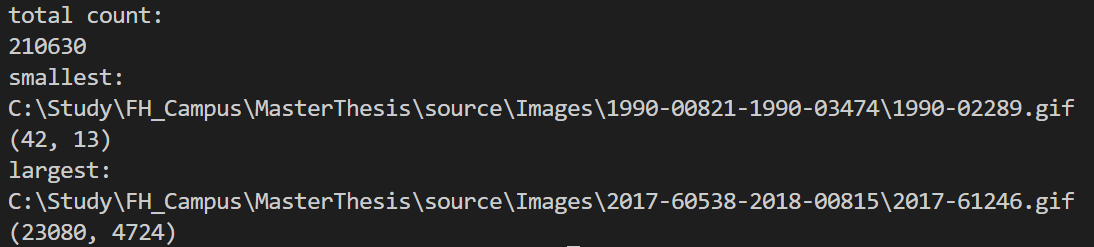
\includegraphics[height=3.5cm]{images/data_smallest_largest.png}
	\caption{Ergebnis Ermittlung kleinstes und größtes Bild}
	\label{fig:data_smallest_largest}
\end{figure}
Das kleinste Bild hat 42 mal 13 Pixel und wie in Abbilung \ref{fig:data_smallest} zu sehen ist, kann man hier die Pixel einzeln abzählen.
\begin{figure}[htbp]
	\centering
		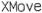
\includegraphics[height=1cm]{images/data_smallest.png}
	\caption{Kleinstes Bild im Datensatz}
	\label{fig:data_smallest}
\end{figure}
Das größte Bild ist 23080 mal 4724 Pixel groß, was für Latex leider zu groß war und ich es runterkomprimieren musste.
Das komprimierte Bild ist in Abbildung \ref{fig:data_largest} veranschaulicht.
\begin{figure}[htbp]
	\centering
		
\includegraphics[height=3.5cm]{images/data_largest_screenshot_full.png}
	\caption{Größtes Bild im Datensatz}
	\label{fig:data_largest}
\end{figure}
Der Datensatz weist eine hohe diversität bei den Merkmalen Größe, Auflösung, Ausrichtung und Farben auf wie auch in Abbildung \ref{fig:data_inside_folder} zu sehen ist.
Es sind kleine und große, horizontale und vertikale, farbig und schwarz weis Bilder vorhanden.
Ebenfalls gibt es Markenlogos die ausschließlich aus Text bestehen, ein Logo in Bildform und Text beinhalten oder nur ein Logo in Bildform enthalten.

\section{Bildvorverarbeitung}
\label{sec:imagepreprocessing}
\subsection{Sift}
Da SIFT gegenüber Skalierung und Rotation invariant ist wird hierbei keine Bildvorerarbeitung benötigt (siehe Kapitel \ref{sift}).
\subsection{Siamese Network}
Aufgrund der diversität zwischen den Bildern im Datensatz benötigt es für das Siamesische Netzwerk eine Bildvorverarbeitung.
Hierfür wurde eine Hilfsfunktion (siehe Listing \ref{lst:get_average_imagesize}) erstellt, welche den Mittelwert der Breite und Höhe über den kompletten Datensatz berechnet.
\begin{lstlisting}[frame=lines, caption=Hilfsfunktion zur Ermittlung der durchschnittlichen Größe im Datensatz, captionpos=b, label = lst:get_average_imagesize, language=Python, showstringspaces=false]
def get_average_imagesize(filenames):
	widths = []
	heights = []
	for filename in filenames:
		size = PILImage.open(filename, 'r').size
		widths.append(size[0])
		heights.append(size[1])
	average_width = sum(widths)/len(widths)
	average_height = sum(heights)/len(heights)
	return [average_width, average_height]
\end{lstlisting}
Das Ergebnis beträgt gerundet 831 Pixel breit und 505 Pixel hoch ist in Abbildung \ref{fig:data_average_size} zu sehen.
\begin{figure}[htbp]
	\centering
		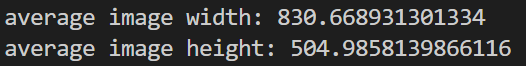
\includegraphics[height=1.5cm]{images/data_average_size.png}
	\caption{Durchschnittliche Größe eines Bildes im Datensatz}
	\label{fig:data_average_size}
\end{figure}
Daraus 

\section{Sift}
\label{sec:sift_implementation}



\newpage
\chapter{Diskussion der Ergebnise}
Vergleich SIFT vs. Simaese Network
skizze: SIFT: benötigt keine Trainignsdaten + keine Bildvorverarbeitung, ist schnell, schlechte generalisierung, simple implementierung
Siamese Network (mit CNN): benötigt Trainingsdaten um zu lernen, benötigt Bildvorverarbeitung, viele Parameter zu setzen
\begin{table*}[htbp]
	\centering
		\begin{tabular}{|c|c|m{20em}|}
		\hline
		\rowcolor[gray]{0.9}
		Algorithmus & Vorteile & Nachteile \\
		\hline
		SIFT & tbd. VORTEILE & tbd. NACHTEILE  \\
		Siamese Network & tbd. VORTEILE & tbd. NACHTEILE  \\
		\hline	
		\end{tabular}
	\caption{Vergleich SIFT vs. Simaese Network}
	\label{tab:siftvssiamese}
\end{table*}

\newpage
\chapter{Conclusio}

\newpage
\chapter{Ausblick}

\newpage


%\chapter{Examples}
%\label{chap:intro}
%Textkörper mit Bild
%
%\begin{figure}[htbp]
%	\centering
%		
\includegraphics[height=5cm]{images/buecher.png}
%	\caption{Ein Stapel Bücher}
%	\label{fig:buecher}
%\end{figure}
%
%
%Textkörper Fortsetzung mit Verweis auf den wundervollen Stapel Bücher in Abbildung \ref{fig:buecher}. 
%
%
%\section{Unterkapitel 1}
%\label{sec:Unterkapitel1}
%
%Textkörper mit Formel:
%
%\begin{equation}
%U(j\omega)=\int^{\infty}_{-\infty}{u(t) \cdot e^{-j\omega t}dt}
%\label{form:form1}
%\end{equation}
%
%Textkörper Fortsetzung mit Verweis auf Formel \ref{form:form1}. Und nicht zu vergessen: es gibt auch noch eine tolle Abbildung in Kapitel \ref{chap:intro}, nämlich Abbildung \ref{fig:buecher}. 
%
%
%\subsection{Unter-Unterkapitel 11}
%\label{sec:UnterUnterkapitel11}
%
%Textkörper mit direktem Zitat und Seitenanzahl:
%``It would be very easy to show how technical or report writing differed from other writing'' \cite[p.~3]{young2002technical}.
%
%\subsection{Unter-Unterkapitel 12}
%\label{sec:UnterUnterkapitel12}
%
%Textkörper mit Referenzen:
%Für weiterführende Informationen zum wissenschaftlichen Schreiben siehe "J. Schimel, Writing Science" \cite{schimel2012writing}. Es wird empfohlen den Sprachleitfaden der FH Campus Wien \cite{alker2006} zu berücksichtigen und die Checkliste für wissenschafltiches Schreiben \cite{petz2018} zu verwenden. Beide Leitfäden sind im FH Portal zu finden.
%
%\chapter{Kapitel 2}
%\label{chap:back}
%
%Textkörper mit noch einem Bild
%
%\begin{figure}[htbp]
%	\centering
%		
\includegraphics{images/birne}
%	\caption{Eine Glühbirne}
%	\label{fig:birne}
%\end{figure}
%
%
%
%\section{Unterkapitel 21}
%\label{sec:Unterkapitel21}
%
%Textkörper mit Tabelle.
%
%\begin{table*}[htbp]
%	\centering
%		\begin{tabular}{|l|c|r|}
%		\hline
%		\rowcolor[gray]{0.9}
%		Spalte 1 & Spalte 2 & Spalte 3 \\
%		\hline
%		Affen & Giraffen & Löwen \\
%		Apfel & Birnen & Bananen \\
%		Irgend & et & was \\
%		\hline	
%		\end{tabular}
%	\caption{Beispiel für eine Tabelle}
%	\label{tab:BeispielFuerEineTabelle}
%\end{table*}
%
%Man beachte die Gegenüberstellung in Tabelle \ref{tab:BeispielFuerEineTabelle}.
%
%%Online Tabellengenerator für Latex: https://www.tablesgenerator.com/
%
%\section{Unterkapitel 23}
%\label{sec:Unterkapite23}
%
%Aufzählungen:
%
%Nummeriert:
%
%\begin{enumerate}
%	\item Punkt 1
%	\item Punkt 2
%\end{enumerate}
%
%Mit Bullet Points:
%
%\begin{itemize}
%	\item Punkt 1
%	\item Punkt 2
%\end{itemize}
%
%Mit Beschreibungen:
%
%\begin{description}
%	\item[Item 1] das ist der 1.Punkt
%	\item[Item 2] und das der 2.
%\end{description}
%
%
%Auch Programmcodes können an entsprechender Stelle eingefügt werden, man beachte dazu auch Listing \ref{lst:conv}.
%
%% see also http://mirror.easyname.at/ctan/macros/latex/contrib/listings/listings.pdf for options
%
%\begin{lstlisting}[frame=lines, caption=Simple Listing, captionpos=b, label = lst:conv, language=C, showstringspaces=false]
%#include <stdio.h>
%int main()
%{
%	int i, n, t1 = 0, t2 = 1, nextTerm;
%
%	printf("Enter the number of terms: ");
%	scanf("%d", &n);
%
%	printf("Fibonacci Series: ");
%
%	for (i = 1; i <= n; ++i)
%	{
%		printf("%d, ", t1);
%		nextTerm = t1 + t2;
%		t1 = t2;
%		t2 = nextTerm;
%	}
%	return 0;
%}
%\end{lstlisting}
%
%Und zuguterletzt, Formeln mitten im Fliesstext, wie z.B. $a^2+b^2=c^2$, in einem Absatz.

%\newpage
%\chapter{Related Work}


% --- Bibliography ------------------------------------------------------

%IEEE Citation [1]
\bibliographystyle{IEEEtran}
%for alphanumeric citation eg.: [ABC19]
%\bibliographystyle{alpha}

% List references I definitely want in the bibliography,
% regardless of whether or not I cite them in the thesis.

\newpage
\addcontentsline{toc}{chapter}{Bibliographie}
\bibliography{testBib}

\newpage

% --- List of Figures ----------------------------------------------------

\addcontentsline{toc}{chapter}{Abbildungen}
\listoffigures


% --- List of Tables -----------------------------------------------------

\newpage
\addcontentsline{toc}{chapter}{Tabellen}
\listoftables

% --- Appendix A -----------------------------------------------------

\newpage
\appendix
\backmatter
\begin{appendices}
\chapter{Appendix}
\begin{lstlisting}[frame=lines, caption=Vollständiger Code für ein neuronales Netzwerk das Handschriftliche Zahlen erkennt, captionpos=b, label = lst:mnist_example, language=Python, showstringspaces=false]
import keras
from tensorflow.keras.datasets import mnist
from matplotlib import pyplot as plt
from keras.layers import Dense
from keras.models import Sequential

# load dataset
(pic_train, label_train), (pic_test, label_test) = mnist.load_data()
# summarize loaded dataset
print('Train: X=%s, y=%s' % (pic_train.shape, label_train.shape))
print('Test: X=%s, y=%s' % (pic_test.shape, label_test.shape))
# plot first few images
fig, axes = plt.subplots(ncols=5, sharex=False, 
    sharey=True, figsize=(10, 4))
for i in range(5):
    axes[i].set_title(label_train[i])
    axes[i].imshow(pic_train[i], cmap='gray')
    axes[i].get_xaxis().set_visible(False)
    axes[i].get_yaxis().set_visible(False)
plt.show()

num_classes = 10 # Zahlen von 0 bis 9
image_size = 28*28 # Pixels

# Gives a new shape to an array without changing its data.
x_train = pic_train.reshape(pic_train.shape[0], image_size)
x_test = pic_test.reshape(pic_test.shape[0], image_size)

# Converts a class vector (integers) to binary class matrix.
y_train = keras.utils.np_utils.to_categorical(label_train, num_classes)
y_test = keras.utils.np_utils.to_categorical(label_test, num_classes)

model = Sequential()

model.add(Dense(units=15, activation='sigmoid', input_shape=(image_size,)))
model.add(Dense(units=num_classes, activation='softmax'))
model.summary()

model.compile(loss='categorical_crossentropy', optimizer='sgd',metrics=['acc']) 
history = model.fit(x_train, y_train, batch_size=128, epochs=5, verbose=False, validation_split=.1)
loss, accuracy  = model.evaluate(x_test, y_test, verbose=False)

plt.plot(history.history['acc'])
plt.plot(history.history['val_acc'])
plt.title('model accuracy')
plt.ylabel('accuracy')
plt.xlabel('epoch')
plt.legend(['training', 'validation'], loc='best')
plt.show()

print(f'Test loss: {loss:.3}')
print(f'Test accuracy: {accuracy:.3}')
\end{lstlisting}

\clearpage
\end{appendices}

\end{document}
